% Options for packages loaded elsewhere
\PassOptionsToPackage{unicode}{hyperref}
\PassOptionsToPackage{hyphens}{url}
\PassOptionsToPackage{dvipsnames,svgnames,x11names}{xcolor}
\documentclass[
  10pt,
]{article}
\usepackage{xcolor}
\usepackage[margin=2.5cm]{geometry}
\usepackage{setspace}
\doublespacing
% Code/IR listings (pandoc verbatim): shrink to \small and single-space so
% wide IR dumps fit the thesis-width margins without per-line trimming.
\makeatletter
\g@addto@macro\@verbatim{\small\setstretch{1}}
\makeatother
\usepackage{amsmath,amssymb}
\setcounter{secnumdepth}{-\maxdimen} % remove section numbering
\usepackage{iftex}
\ifPDFTeX
  \usepackage[T1]{fontenc}
  \usepackage[utf8]{inputenc}
  \usepackage{textcomp} % provide euro and other symbols
\else % if luatex or xetex
  \usepackage{unicode-math} % this also loads fontspec
  \defaultfontfeatures{Scale=MatchLowercase}
  \defaultfontfeatures[\rmfamily]{Ligatures=TeX,Scale=1}
\fi
\usepackage{lmodern}
\ifPDFTeX\else
  % xetex/luatex font selection
\fi
% Use upquote if available, for straight quotes in verbatim environments
\IfFileExists{upquote.sty}{\usepackage{upquote}}{}
\IfFileExists{microtype.sty}{% use microtype if available
  \usepackage[]{microtype}
  \UseMicrotypeSet[protrusion]{basicmath} % disable protrusion for tt fonts
}{}
\makeatletter
\@ifundefined{KOMAClassName}{% if non-KOMA class
  \IfFileExists{parskip.sty}{%
    \usepackage{parskip}
  }{% else
    \setlength{\parindent}{0pt}
    \setlength{\parskip}{6pt plus 2pt minus 1pt}}
}{% if KOMA class
  \KOMAoptions{parskip=half}}
\makeatother
\usepackage{longtable,booktabs,array}
\newcounter{none} % for unnumbered tables
\usepackage{calc} % for calculating minipage widths
% Correct order of tables after \paragraph or \subparagraph
\usepackage{etoolbox}
\makeatletter
\patchcmd\longtable{\par}{\if@noskipsec\mbox{}\fi\par}{}{}
\makeatother
% Allow footnotes in longtable head/foot
\IfFileExists{footnotehyper.sty}{\usepackage{footnotehyper}}{\usepackage{footnote}}
\makesavenoteenv{longtable}
\usepackage{graphicx}
\makeatletter
\newsavebox\pandoc@box
\newcommand*\pandocbounded[1]{% scales image to fit in text height/width
  \sbox\pandoc@box{#1}%
  \Gscale@div\@tempa{\textheight}{\dimexpr\ht\pandoc@box+\dp\pandoc@box\relax}%
  \Gscale@div\@tempb{\linewidth}{\wd\pandoc@box}%
  \ifdim\@tempb\p@<\@tempa\p@\let\@tempa\@tempb\fi% select the smaller of both
  \ifdim\@tempa\p@<\p@\scalebox{\@tempa}{\usebox\pandoc@box}%
  \else\usebox{\pandoc@box}%
  \fi%
}
% Set default figure placement to htbp
\def\fps@figure{htbp}
\makeatother
\setlength{\emergencystretch}{3em} % prevent overfull lines
\providecommand{\tightlist}{%
  \setlength{\itemsep}{0pt}\setlength{\parskip}{0pt}}
\usepackage{bookmark}
\IfFileExists{xurl.sty}{\usepackage{xurl}}{} % add URL line breaks if available
\urlstyle{same}
\hypersetup{
  colorlinks=true,
  linkcolor={Maroon},
  filecolor={Maroon},
  citecolor={Blue},
  urlcolor={Blue},
  pdfcreator={LaTeX via pandoc}}

\author{}
\date{}

\begin{document}

% ---------------------------------------------------------------------------
% Title page
% ---------------------------------------------------------------------------
\begin{titlepage}
\centering
\vspace*{2cm}

{\LARGE\bfseries Imperial College London\par}
\vspace{0.5cm}
{\large Department of Electrical and Electronic Engineering\par}

\vspace{3cm}

{\Huge\bfseries Accelerating the Open-Sora MMDiT\\[4mm]
Structure on PLENA by a TileLang Compiler\par}

\vspace{2.5cm}

{\Large Ziqian Gao\par}

\vfill

{\large 2026-06-07\par}
\vspace{1cm}
\end{titlepage}

{
\setcounter{tocdepth}{3}
\tableofcontents
}

\subsection*{Abstract}\label{abstract}

This work delivers two things. First, we built a \textbf{TileLang
compiler} for PLENA with strong compatibility: a kernel written in the
ordinary GPU TileLang style runs as-is, with no changes, and on top of
that compatibility the compiler performs aggressive memory-access and
compute fusion --- so the generated code is highly efficient. Second,
using only this compiler, we fully accelerated the heaviest part of
Open-Sora, the \textbf{MMDiT} backbone, \emph{without a single line of
hand-written ISA or any PLENA-specific adaptation}: we wrote plain
TileLang exactly as one would for a GPU, and the compiler did the rest.

Why MMDiT is worth this effort. Its difficulty is of a different kind
from an LLM's. The structure is extremely regular, so it never runs into
the autoregressive-decode and KV-cache problems that dominate LLM
serving --- but its compute cost is enormous, on the order of
\textbf{150× that of a similarly sized LLM}. This cost is precisely why
video-generation systems of this class (e.g.\ OpenAI-style Sora models)
are so expensive to run. At the same time MMDiT is a remarkably powerful
and general structure: the same backbone is used in robotics
\textbf{VLA} models. In other words, MMDiT is a highly capable structure
with an extremely high compute bill --- so bringing its time cost and
energy cost down to roughly \textbf{one third} of the original turns it
into a genuinely valuable result, and one that transfers well beyond
video generation.

The value of the TileLang compiler is twofold. It keeps the development
cost low --- there is no need to hand-write ISA or maintain a bespoke
per-chip kernel library --- while still hitting high efficiency. And it
guarantees \textbf{compatibility}, whose importance is a major issue in
industry yet is badly underestimated in academia. When a chip ---
especially an unconventional architecture like a GPU or a TPU --- comes
back from the fab, only half the job is done. A chip is only as usable as
the software that can target it: without a compiler that lets existing
code run without rewrites, the cost of adopting the chip falls entirely
on every team that wants to use it, and most simply will not pay it. In
practice a good, compatible compiler is often \emph{more} decisive than
raw peak performance --- it is what determines whether a chip can be
adopted at scale at all, rather than remaining a one-off that only its
designers can program. This report describes both the compiler and the
MMDiT acceleration it enabled.

\begin{center}\rule{0.5\linewidth}{0.5pt}\end{center}

\section{Part I --- The TileLang Compiler}\label{part-compiler}

\subsection{1. ISA Compiler}\label{isa-compiler}

\subsubsection{1.1 Introduction}\label{isa-compiler-introduction}

The ISA compiler is the toolchain that lowers a kernel written in
\textbf{TileLang} down to the PLENA instruction set. TileLang is a
tile-based domain-specific language for expressing tensor programs: the
programmer reasons in terms of tiles of data and the parallel operations
over them, rather than in terms of individual scalar threads or
hand-placed memory transfers.

To understand what our compiler has to do --- and what it deliberately
avoids doing --- it helps to first recall how TileLang is normally
compiled. The canonical TileLang pipeline targets NVIDIA GPUs and
proceeds in stages: TileLang is first lowered to \textbf{TVM IR}, which
is then emitted as \textbf{CUDA} C++; the CUDA source is handed to
NVIDIA's compiler, which lowers it through \textbf{LLVM} and finally to
\textbf{PTX} for execution on the GPU. Every layer of this stack is
built around the GPU execution model, and as a result it is very hard to
escape the assumptions of that model: the whole path is fundamentally a
\textbf{SIMT} (single-instruction, multiple-thread) abstraction ---
many threads, grouped into warps and blocks, each with its own program
counter and register state. PLENA, by contrast, is a \textbf{SIMD}
(single-instruction, multiple-data) machine: a single instruction stream
drives wide vector and tile datapaths, with no per-thread divergence and
no warp scheduler. Bridging this gap --- taking a program written in a
SIMT-flavored language and mapping it efficiently onto a SIMD
architecture --- is the central problem our compiler solves.

Our compiler is built to satisfy two core requirements.

\begin{enumerate}
\def\labelenumi{\arabic{enumi}.}
\item
  \textbf{Compatibility.} We try as hard as possible \emph{not} to make
  the user learn new syntax. The ideal is that someone who knows nothing
  about the specifics of the PLENA hardware --- who only knows how to
  write TileLang and is only familiar with the SIMT execution model ---
  can move onto our compiler seamlessly, with no rewriting. This matters
  in practice, not just in principle: in our experience the SIMT style is
  \emph{far} easier to write than SIMD, and it is also far easier to
  optimize. Preserving that programming experience is a feature, not a
  compromise.
\item
  \textbf{Performance.} Subject to the first requirement, the generated
  code should be as fast as possible. At a minimum it must beat
  hand-written code. We achieve this primarily through two forms of
  fusion: \textbf{compute fusion} (merging arithmetic operations to keep
  data in the datapath) and \textbf{memory-access fusion} (merging loads
  and stores to use the memory system efficiently). Both are described in
  detail in the sections that follow.
\end{enumerate}

\subsubsection{1.2 Hardware Architecture
Mapping}\label{isa-compiler-hardware-architecture-mapping}

A defining property of TileLang is that it \textbf{exposes the hardware}
to the programmer. This is precisely what sets TileLang apart from a
language like Triton: where Triton hides the memory hierarchy and
scheduling behind a high-level tile abstraction, TileLang makes the
underlying hardware structure --- the memory levels, the placement of
tiles, the parallel execution units --- visible in the program itself.
The kernel is written against a concrete picture of the machine, not an
abstract one.

This property is double-edged. Because the hardware is exposed, and
because the hardware that TileLang programs are normally written against
is a GPU, the source program carries GPU-architecture assumptions baked
directly into it. To run such a program on PLENA we therefore need a way
to \textbf{map the GPU architecture onto the TPU architecture} --- to
take the GPU-shaped structure that TileLang exposes and re-interpret it
in terms of PLENA's units. This is genuinely challenging: the two
machines do not have a one-to-one correspondence between their memory
levels or their execution models.

But the same property that creates the difficulty also creates the
opportunity. Because TileLang has already made the hardware structure
explicit in the program, the mapping problem is not a vague semantic
recovery task --- the structure we need to re-target is right there in
the source. The exposed hardware that forces us to do the mapping is
also exactly what gives us a concrete handle to do it with.

The concrete mapping is, in fact, very simple. PLENA has \textbf{four
local storage units}: FPRAM, vector RAM (VRAM), matrix RAM (MRAM), and
integer RAM. Integer RAM exists only to absorb spills of the integer
registers; it plays no role in the data layout and we set it aside here
(it is covered later, in the SCF-to-ISA generation stage). The three
units that matter for placement are \textbf{FPRAM}, \textbf{VRAM}, and
\textbf{MRAM}, and we map the TileLang memory scopes onto them as
follows:

\begin{longtable}[]{@{}ll@{}}
\toprule\noalign{}
TileLang scope & PLENA unit \\
\midrule\noalign{}
\endhead
\bottomrule\noalign{}
\endlastfoot
\texttt{shared} memory & MRAM and VRAM \\
2D \texttt{fragment} & VRAM \\
1D \texttt{fragment} / \texttt{local} & FPRAM \\
\end{longtable}

That is, \texttt{shared} memory is treated as storage living in MRAM and
VRAM; a 2D fragment is treated as storage in VRAM; and a 1D fragment or
a \texttt{local} buffer is treated as storage in FPRAM.

\begin{figure}
\centering
% TODO: figure illustrating the GPU-scope -> PLENA-unit mapping
\caption{Mapping of TileLang memory scopes onto PLENA storage units}
\end{figure}

Under this mapping the GPU memory-movement idioms carry over directly.
The transfer from HBM into MRAM and VRAM is exactly what, on an H100,
would be the DMA from \textbf{global} memory into \textbf{shared}
memory. By making the correspondence line up at this level, we preserve
compatibility with the mainstream programming model: a kernel written in
the usual global-to-shared style needs no change to run on PLENA. This
is the rough shape of the idea; the sections that follow make each piece
precise.

\subsubsection{1.3 Frontend}\label{isa-compiler-frontend}

The frontend has two jobs above all others, and they are exactly the two
forms of fusion introduced earlier: \textbf{compute fusion} and
\textbf{memory-access fusion}.

\paragraph{Compute fusion}\label{frontend-compute-fusion}

Compute fusion means turning SIMT-style parallelism into native SIMD
operations. There are two patterns:

\begin{itemize}
\tightlist
\item
  A \texttt{parallel} loop --- which in the SIMT model is a fan-out of
  many independent threads, each doing one scalar's worth of work ---
  must be collapsed into a single \textbf{vector} operation that does
  the whole row at once.
\item
  Multiple separate GEMMs must be merged into one large
  \textbf{matrix-multiply}, so the matrix datapath is driven with one
  wide instruction instead of many small ones.
\end{itemize}

In both cases the idea is the same: take the many small units of work
that the SIMT source expresses and collapse them into one wide datapath
operation.

\paragraph{Memory-access fusion and block
fusing}\label{frontend-memory-access-fusion}

Memory-access fusion means coalescing many narrow DMAs into one large
DMA. On top of this, because of the coarse granularity of the TPU
hardware, the frontend must implement the operation that is both the
single most important one in the whole compiler and the one for which
the off-the-shelf TVM libraries offer the least support: \textbf{block
fusing}.

The essence of block fusing is this. The TPU's hardware granularity is
very coarse, so to keep the datapath full we must merge work \emph{across
multiple block IDs} rather than treating each block independently. On a
GPU this need barely arises: a GPU has a deep, multi-level cache
hierarchy that already delivers much of the effect of memory-access
coalescing for free, so the stock TVM libraries contain very little
machinery for it. Our TPU has no such cache hierarchy --- so we must
perform that coalescing explicitly, in the compiler. The mechanism is to
partition the block IDs into groups and fuse each group into a single
\textbf{cluster}.

\paragraph{Why this is necessary --- a flash-attention
example.}\label{frontend-why-block-fusing}

Take flash attention as the running example. The baseline storage format
is the standard \textbf{BSHD} layout (batch, sequence, heads, head-dim).
The relevant hardware number is \texttt{VLEN} --- which on PLENA is
simultaneously the \textbf{memory bandwidth} and the \textbf{maximum
vector width} --- and it is around \textbf{1024}. The head dimension,
however, is typically \textbf{128}: only one eighth of \texttt{VLEN}.

If we naively map one head onto the datapath, each vector instruction and
each DMA carries 128 useful elements out of a possible 1024. In other
words \textbf{7/8 of both the memory bandwidth and the vector utilization
is wasted}, and the machine runs at one eighth of its peak. This is
completely unacceptable.

\begin{figure}
\centering
% TODO: figure -- one head (128) occupying 1/8 of a 1024-wide VLEN lane,
% vs. eight heads packed by clustering to fill the full 1024 width.
\caption{Head-dim 128 underfills a 1024-wide datapath; clustering eight
block IDs fills it}
\end{figure}

There are two ways to deal with this:

\begin{enumerate}
\def\labelenumi{\arabic{enumi}.}
\item
  \textbf{Force the user to write 3D shared-memory tiles.} An earlier
  runtime compiler of ours took exactly this route --- the user writes a
  third tile dimension explicitly so that several heads are packed into
  one wide tile by hand. Both to develop and to use, the verdict was
  that it is very hard to write: a 2D tile is always closer to human
  intuition than a 3D one. Worse, to make the 3D form work you end up
  writing a great many specialized instructions, which drifts the whole
  project further and further from the community --- more and more
  reinventing the wheel behind closed doors. We give this
  runtime-compiler example in the appendix and show briefly why the
  direction is both hard to write and hard to use.
\item
  \textbf{Let the compiler do the whole job.} The user writes in the
  most basic, simplest, most mainstream-aligned way --- a plain 2D tile,
  one head, exactly as they would on a GPU --- and the fusion of block
  IDs into clusters is performed automatically by the compiler. For the
  flash-attention case above, the compiler groups eight block IDs (eight
  heads) into one cluster so that all 1024 lanes are filled and no
  bandwidth is wasted, without the user ever writing a 3D tile.
\end{enumerate}

We take the second route, and it is the single most central task of the
frontend. The rest of this subsection describes the IR pipeline that
carries it out, again using flash attention as the example.

\paragraph{IR pass architecture.}\label{frontend-ir-pass-architecture}

The frontend is a chain of small passes. A user kernel enters as a
\texttt{tilelang} \texttt{PrimFunc} (a TIR program), is lowered through a
sequence of intermediate representations, and exits as an
\textbf{HLIR} module --- a flat list of PLENA ops over physically-scoped
buffers --- that the backend consumes. The overall flow is:

\begin{verbatim}
   tilelang PrimFunc  (raw TIR: T.copy / T.gemm / T.Parallel / T.reduce)
        |
        |  (0) Stmt prep        inline_let . fission_vector_chains
        |                       . split_btmm . lower_compound_fp_stores
        |                       . hoist_float_constants
        v
   TIR  (one-op-per-loop form; FP literals hoisted to global.fpram)
        |
        |  (1) mid_ir pipeline
        |    infer_lane_axis    pick the lane (block-id) axis from usage
        |    fold               raw TIR shapes -> mid_ir nodes
        |                       (Dma / Gemm / Elementwise / Reduce)
        |    mark               tag each op with its lane-fusion role
        |    split              split lane axis -> (number, phase);
        |                       grow on-chip buffers by a CLUSTER dim   <-- block fusing
        |    distribute_cluster push CLUSTER axes inside unroll loops
        |    async_wrap         wrap each can-async op in an Async region
        |    view               assign per-ref view_perm (BSHD / BHSD)
        |    fuse               collapse each Async into one MultiLaneOp
        |    burn_view          bake the soft view into physical shape
        |    to_plena           mid_ir -> HLIR  (the only pass to leave mid_ir)
        v
   HLIR  (plena.* ops; lane-expanded buffers; tilelang scopes)
        |
        |  (1.25) loop_interchange <-> fuse_adjacent_loops  (to fixed point)
        |  (1.5)  dead_buffer_elim
        v
   HLIR  -> backend (address allocation, ISA emit)
\end{verbatim}

Two stages are worth calling out, because they are where the two fusions
from above actually happen.

\textbf{Where compute fusion happens --- \texttt{fold}.} The \texttt{fold}
pass is what collapses the many small SIMT-shaped statements into single
wide operations. A \texttt{T.Parallel} loop of per-element stores folds
to one \texttt{Elementwise} node; a \texttt{T.gemm} folds to one
\texttt{Gemm} node; a \texttt{T.reduce} to one \texttt{Reduce}. After
\texttt{fold}, the body is a clean sequence of whole-tile ops rather than
a nest of scalar loops --- this is compute fusion made concrete in the
IR.

\textbf{Where block fusing happens --- \texttt{split} and the cluster
passes.} \texttt{infer\_lane\_axis} first identifies which block-id axis
is the lane axis (the one that appears as a bare index into a buffer,
e.g.\ the head index \texttt{by} in \texttt{Q[0, \dots, by, 0]}).
\texttt{split} then divides that axis into a \emph{number} part (a
smaller hardware grid) and a \emph{phase} part of size
\texttt{cluster\_count} --- the \textbf{CLUSTER} axis whose lanes run in
lockstep --- and grows every on-chip buffer by one outer dimension of
size \texttt{cluster\_count}. In the flash-attention example,
\texttt{cluster\_count = 8} packs eight heads (8 × 128 = 1024) into one
cluster so the full datapath is filled. The remaining cluster passes
(\texttt{distribute\_cluster}, \texttt{async\_wrap}, \texttt{view},
\texttt{fuse}, \texttt{burn\_view}) carry that cluster structure down to
single multi-lane HW instructions. This is exactly the automatic
block-id fusion promised above: the user wrote a plain 2D, one-head
kernel, and the compiler turned it into a cluster of eight without a
single 3D tile in the source.

The walkthrough below traces flash attention through these stages in
detail.

\paragraph{Worked example: flash attention through the
passes.}\label{frontend-fa-walkthrough}

To make each pass concrete we trace the actual flash-attention kernel
that the MMDiT pipeline compiles, showing the IR before and after every
pass. The two things to watch are (i) how the \textbf{cluster dimension}
is introduced and then propagated through every buffer and index, and
(ii) how each buffer's \textbf{layout} (the position of the lane axis) is
chosen so that the hardware op it feeds sees the data in the order it
needs.

The source is plain GPU-style TileLang. The grid is
\texttt{T.Kernel(num\_q\_blocks, head\_count) as (q\_block, by)}; every
on-chip buffer is a per-head 2D (or 1D) tile, and the author never fuses
heads by hand:

\begin{verbatim}
  with T.Kernel(num_q_blocks, head_count) as (q_block, by):
      head = by
      Q_sh   = T.alloc_shared((rows, hlen), "float16")   # (1024, 128)
      K_sh   = T.alloc_shared((rows, hlen), "float16")   # (1024, 128)  gemm RHS
      V_sh   = T.alloc_shared((rows, hlen), "float16")   # (1024, 128)  matmul RHS
      S_loc  = T.alloc_fragment((rows, MLEN), "float16") # (1024, 1024)
      O_loc  = T.alloc_fragment((rows, hlen), "float16") # (1024, 128)
      M_OLD  = T.alloc_fragment((rows,), "float16")      # (1024,)  1-D fp state
      M_CURR = T.alloc_fragment((rows,), "float16")      # (1024,)
      ...
      T.copy(Q_hbm[0, q_block*rows:(q_block+1)*rows, head, 0:hlen], Q_sh)
      for kv_block in T.serial(num_kv_blocks):
          T.copy(K_hbm[0, kv_block*rows:(kv_block+1)*rows, head, 0:hlen], K_sh)
          T.copy(V_hbm[0, kv_block*rows:(kv_block+1)*rows, head, 0:hlen], V_sh)
          with T.attr(0, KIND, "btmm"):
              T.gemm(Q_sh, K_sh, S_loc, transpose_B=True)   # Q @ K^T
          for row in T.serial(rows):
              for col in T.Parallel(MLEN):
                  S_loc[row, col] = S_loc[row, col] * T.float16(scale_val)
          T.reduce_max(S_loc, M_CURR, dim=1, clear=False)    # online softmax
          ...
          T.gemm(S_loc, V_sh, PV_loc)                        # P @ V (per head)
          for row in T.serial(rows):
              for col in T.Parallel(hlen):
                  O_loc[row, col] = O_loc[row, col] + PV_loc[row, col]
\end{verbatim}

For the MMDiT geometry \texttt{rows = MLEN = 1024}, \texttt{hlen = 128},
and there are \texttt{24} heads, so \texttt{head\_count = 24} and the
hardware lane width is \texttt{MLEN / hlen = 8}. We now take the passes
one at a time.

\subparagraph{(0) Stmt prep.}\label{fa-stmt-prep} The first group of
passes are plain TIR-to-TIR rewrites that run before the mid-IR exists;
they normalise the program so the later folding rules match.
\texttt{inline\_let} removes \texttt{let} bindings; \texttt{fission\_%
vector\_chains} breaks a compound vector right-hand side (e.g.\ a fused
\texttt{a*b+c}) into one elementary op per loop, because the mid-IR
\texttt{fold} pass matches exactly one operation per loop body;
\texttt{split\_btmm} inserts the deferred \texttt{M\_BMM\_WO} drain after
the K-loop (the BTMM hardware accumulates each \texttt{k\_block} and one
drain writes the result out); \texttt{lower\_compound\_fp\_stores} does
the analogous one-op-per-store rewrite for scalar FPRAM chains. Finally
\texttt{hoist\_float\_constants} lifts every float literal into an
auto-synthesised one-slot \texttt{global.fpram} buffer. The two literals
in this kernel --- the softmax scale \texttt{1/sqrt(128) = 0.0883883} and
the \texttt{-1e4} ``\texttt{-inf}'' surrogate --- become:

\begin{verbatim}
  T.float16(scale_val)   -->  __const_f16_0p0883883 : float16() @global.fpram
  T.float16(-1.0e4)      -->  __const_f16_neg10000  : float16() @global.fpram
\end{verbatim}

so the author never declares or preloads them. At the end of stmt prep
the program is still ordinary TIR, but every loop body holds exactly one
op and every constant is a named FPRAM buffer.

\subparagraph{(1) \texttt{infer\_lane\_axis} --- pick the lane
axis.}\label{fa-infer-lane} \emph{What it does:} chooses which grid axis
becomes the lane (cluster) axis. \emph{How:} it walks every
\texttt{BufferLoad} and every \texttt{tl.tileop.region} call and asks,
for each grid var, whether it ever appears as a \textbf{bare} index slot
--- the var itself sitting directly in an index position, rather than
only inside offset-arithmetic. The contrast it is drawing is between a
var used as an \emph{indexing} dimension and one used only to compute an
\emph{offset}: here \texttt{by} (the head) indexes directly in
\texttt{Q\_hbm[0, \dots, head, 0]}, while \texttt{q\_block} appears only
inside the offset \texttt{q\_block*rows} (a \texttt{Mul}). A bare grid
var whose extent is divisible by the lane width is a lane candidate;
\texttt{by} is the only one, so it is selected and recorded on the
function:

\begin{verbatim}
  MidFunc.lane_axes = ['head']        # (q_block stays an ordinary outer grid loop)
\end{verbatim}

This is the \texttt{lane\_axes = ['head']} line in the final mid-IR
header. No buffer shape changes yet --- this pass only annotates.

It is worth being precise about the scope of the ``bare'' test, because
it is narrower than the index machinery elsewhere in the frontend.
\texttt{infer\_lane\_axis} is only a \emph{selection heuristic}, run on
raw TIR before \texttt{fold} exists, and it accepts a grid var as a lane
candidate only when the index slot is literally that \texttt{tir.Var}.
The mid-IR index representation itself is far more general: an index is
any \texttt{IndexExpr} --- an integer, a \texttt{VarRef}, a whole-axis
\texttt{Slice}, or a compound \texttt{\{op, args\}} expression such as
\texttt{\{add: [VarRef, const]\}} or \texttt{\{mul: [VarRef, stride]\}}.
These compound forms are built in \texttt{fold} (which turns any TIR
\texttt{Add}/\texttt{Mul} index into the corresponding compound node) and
in \texttt{view}, which is exactly where the reconstructed lane index
\texttt{head\_phase + head\_number * cluster\_count} is synthesised.\footnote{So
\texttt{var + constant} \emph{is} a fully supported index form
everywhere downstream; the only place that insists on a literal var is
the lane-axis picker. One practical consequence: if a kernel indexes its
lane dimension only as \texttt{head + offset} with a non-zero constant
(e.g.\ an output written into a head-slice of a wider tensor), that slot
is a \texttt{tir.Add}, not a bare \texttt{Var}, and the auto-picker will
not select it --- the author then supplies
\texttt{T.func\_attr(\{"plena.lane\_axis": "head"\})} to name it
explicitly. In this kernel the output offset \texttt{o\_head\_offset} is
\texttt{0}, so TIR folds \texttt{head + 0} back to the bare
\texttt{head} and the auto-pick succeeds.} In other words, the strict
bare-var rule governs only \emph{which axis to fuse}; it does not
restrict the index arithmetic the compiler can represent or generate.

\subparagraph{(2) \texttt{fold} --- raw TIR to mid-IR nodes (compute
fusion).}\label{fa-fold} \emph{What it does:} collapses each recognised
TIR shape into a single typed mid-IR node, which is where SIMT-style
scalar loops become whole-tile operations. \emph{How:} a small pattern
table maps each form to one node:

\begin{verbatim}
  T.copy(region, region)                    -> Dma(src, dst)
  T.gemm(A, B, C) under attr "btmm"          -> Gemm(A, B, C, kind="btmm")
  T.gemm(A, B, C)                            -> Gemm(A, B, C, kind="overwrite")
  for col in T.Parallel(N): d[..,col]=a*b    -> Elementwise(d, [a,b], MUL)
  for col in T.Parallel(N): d[..,col]=exp(a) -> Elementwise(d, [a], EXP)
  T.reduce_max(S, M, dim=1)                  -> Reduce(M, S, MAX, axis=1)
\end{verbatim}

After \texttt{fold} the body is a flat sequence of \texttt{Dma} /
\texttt{Gemm} / \texttt{Elementwise} / \texttt{Reduce} nodes; the scalar
\texttt{for col} loops are gone. Buffer shapes are still the logical 2D
ones the author wrote --- folding does not touch layout.

\subparagraph{(3) \texttt{mark} --- tag each op's lane-fusion
role.}\label{fa-mark} \emph{What it does:} stamps a \texttt{marker} on
every op saying how it participates in lane fusion; later passes consult
this flag rather than re-inspecting the op. \emph{How:} a fixed table:

\begin{verbatim}
  Dma                    -> Marker.DMA          (one multi-lane HW DMA)
  Gemm(kind="btmm")      -> Marker.BTMM         (one multi-lane HW BTMM)
  Gemm(kind="overwrite") -> (no marker)         (per-head P@V, runs in lane loop)
  Elementwise / Reduce   -> Marker.LANE_OP
\end{verbatim}

The \texttt{P\,@\,V} gemm gets \emph{no} marker on purpose: it is a
per-head matmul that will run inside the per-lane loop, not as a fused
multi-lane instruction.

\subparagraph{(4) \texttt{split} --- introduce the cluster dimension
(block fusing).}\label{fa-split} This is the pass that actually performs
block fusing, and it changes two things at once. \emph{What it does
\#1 --- split the grid axis:} the lane axis \texttt{head} is divided into
an outer hardware-grid part and an inner lockstep cluster part:

\begin{verbatim}
  parallel head in 0..24 [blockIdx.y]
    body
        |
        v
  parallel head_number in 0..3 [blockIdx.y]      # 24 / 8 = 3 HW grid steps
    cluster  head_phase  in 0..8  <- head_number  # 8 lanes lockstep = CLUSTER
      body
\end{verbatim}

\texttt{head\_number} keeps the \texttt{blockIdx.y} hardware tag (the
grid simply shrinks from 24 to 3); \texttt{head\_phase} is the new
CLUSTER axis whose \texttt{cluster\_count = 8} lanes execute the body
together. The factor 8 is exactly the lane width \texttt{MLEN/hlen}, and
\texttt{8 × 128 = 1024} is what fills the datapath.

\emph{What it does \#2 --- grow every on-chip buffer by one cluster
dim.} Implemented in \texttt{\_grow\_buffer}: each non-global
\texttt{BufferDef} gets a new outermost dimension of size
\texttt{cluster\_count}, tagged \texttt{cluster\_dim=0} so later passes
can find the lane axis without guessing:

\begin{verbatim}
  Q_sh : (1024, 128)        -> (8, 1024, 128)      cluster_dim=0
  S_loc: (1024, 1024)       -> (8, 1024, 1024)     cluster_dim=0
  M_OLD: (1024,)            -> (8, 1024)     cluster_dim=0, scope->fragment.fpram
\end{verbatim}

A 1-D \texttt{fragment} (per-lane scalar softmax state) has its scope
renamed to \texttt{fragment.fpram} here so that, even though its rank is
now 2, \texttt{to\_plena} still routes it to FPRAM. Crucially,
\texttt{split} does \textbf{not} rewrite the buffer \emph{indices} ---
an existing \texttt{Q\_sh[r, c]} now refers to a rank-3 buffer with a
rank-2 index. That mismatch is intentional and is resolved by
\texttt{view}/\texttt{burn\_view}; deferring it keeps this pass purely
structural.

\subparagraph{(5) \texttt{distribute\_cluster} --- one cluster per
unrolled iter.}\label{fa-distribute} \emph{What it does:} when a CLUSTER
axis encloses an \texttt{unroll}/serial \texttt{for} (here the
\texttt{kv\_block} loop), it pushes the cluster \emph{inside} the loop so
each iteration gets its own cluster body. \emph{Why:} otherwise a single
Async region would appear to span all \texttt{kv\_block} iterations,
whereas the hardware needs each iteration to fire its own DMA / BTMM
dispatch and complete independently.

\begin{verbatim}
  cluster head_phase:                  for kv_block in 0..9:
    for kv_block in 0..9:      -->        cluster head_phase:
      dma K; gemm[btmm] S; ...             dma K; gemm[btmm] S; ...
\end{verbatim}

\subparagraph{(6) \texttt{async\_wrap} --- mark the multi-lane
ops.}\label{fa-async} \emph{What it does:} wraps each \texttt{can\_async}
op (a DMA, a BTMM, or a pure broadcast-free elementwise) in its own
\texttt{Async} region --- one op per Async, the strict ``one async, one
op'' rule. \emph{How / why the split matters:} ops that lower to a single
multi-lane HW instruction (\texttt{M\_BTMM}, the wide vector add, the
wide DMA) are \texttt{can\_async=True} and get wrapped; ops that lower to
\emph{per-row} instructions --- \texttt{Reduce} and any
\texttt{Elementwise} with a \texttt{Broadcast} source (\texttt{S -
M\_CURR}, \texttt{O * M\_RES}) --- are \texttt{can\_async=False} and stay
bare, to be emitted later inside a \texttt{for lane} loop.

\begin{verbatim}
  dma Q ...                 -->   Async { dma Q ... }
  gemm[btmm] S ...          -->   Async { gemm[btmm] S ... }
  reduce[max] M_CURR ...    -->   reduce[max] M_CURR ...   (bare: can_async=False)
\end{verbatim}

\subparagraph{(7) \texttt{view} --- choose each buffer's layout, and
propagate the lane index into HBM.}\label{fa-view} This is where
\textbf{layout} is decided. \emph{What it does:} assigns each on-chip
\texttt{BufferRef} a \texttt{view\_perm} --- a permutation describing
where the lane axis sits in that op's view of the buffer --- from a rule
table keyed on (op-kind, operand position):

\begin{verbatim}
  BTMM output S_loc, and S_loc as P@V LHS  -> BHSD: lane at dim 0  (identity perm)
  everything else (DMA bufs, vector ops)   -> BSHD: lane at dim 1  (perm [1,0,2,..])
\end{verbatim}

The reason for two layouts is that the BTMM hardware writes its result
head-stacked along the row direction (lane outermost, \texttt{BHSD}),
whereas DMAs and vector ops want the lane packed in the column direction
next to the sequence axis (\texttt{BSHD}). Concretely the physical buffer
keeps the lane at storage dim 0, but the op's \emph{view} permutes it:

\begin{verbatim}
  S_loc  (BHSD): viewed as  S_loc[head_phase, row, col]   # lane first
  Q_sh   (BSHD): viewed as  Q_sh[row, head_phase, col]    # lane in the middle
\end{verbatim}

\emph{Second job --- HBM lane substitution.} HBM buffers are global and
are \emph{not} rank-grown; instead, the bare lane var in their index is
replaced by the reconstructed global head index:

\begin{verbatim}
  K_hbm[0, kv_block*1024 : ..., head, 0:128]
        head  -->  head_phase + head_number * 8
  =>  K_hbm[:, (ranged_slice (mul kv_block 1024) 1024),
            (ranged_slice (mul head_number 8) 8), :]  -> K_sh[:, head_phase, :]
\end{verbatim}

So the 8 lanes of one cluster read a contiguous 8-head slice of HBM in a
single DMA. The pass also checks global consistency: if two ops disagreed
on a buffer's view it would raise \texttt{ViewConflictError} (no
auto-reshape today).

\subparagraph{(8) \texttt{fuse} --- collapse each Async into a
\texttt{MultiLaneOp}.}\label{fa-fuse} \emph{What it does:} turns each
\texttt{Async\{one op\}} into a single \texttt{multi\_lane} node that
carries the inner op plus its \texttt{cluster\_axis\_names} and a
\texttt{dim\_map} --- for each lane-aware buffer, which physical dim
corresponds to the cluster axis (here always \texttt{[0]}, since
\texttt{split} put the cluster at dim 0). This is the node that lowers to
one HW instruction over all 8 heads:

\begin{verbatim}
  Async { dma K_hbm[...] -> K_sh[:, head_phase, :] }
      -->
  multi_lane (cluster_axes=['head_phase'], dim_map={'K_sh': [0]}) {
      dma K_hbm[...] -> K_sh[:, head_phase, :]   #dma async
  }
\end{verbatim}

\subparagraph{(9) \texttt{burn\_view} + \texttt{to\_plena} --- bake the
layout and exit to HLIR.}\label{fa-burn} \texttt{burn\_view} makes the
soft per-reference \texttt{view\_perm} hard: it bakes the permutation
into each buffer's single physical shape and rewrites every index tuple
to match (HLIR has no per-ref view). \texttt{to\_plena} is then the only
pass that leaves the mid-IR domain, lowering scopes to physical memories:

\begin{verbatim}
  shared / shared.dyn              -> VRAM (or MRAM for a gemm RHS)
  fragment (rank >= 2)             -> VRAM
  fragment.fpram / 1-D fragment    -> FPRAM
  global.fpram (hoisted consts)    -> FPRAM (prefix stripped)
\end{verbatim}

\subparagraph{The resulting mid-IR.}\label{fa-result} Putting it
together, the final \texttt{midir} makes every decision above directly
readable --- the cluster header, the lane-packed buffer shapes (note
\texttt{S\_loc} with the lane at dim 0 and \texttt{Q\_sh} with it at dim
1), and the split between \texttt{multi\_lane} blocks (one HW instruction
across all eight heads) and bare \texttt{for row} ops (per-lane FP work):

\begin{verbatim}
  // lane_axes = ['head'], cluster_counts = [8]
  allocs:
    Q_sh:  float16(1024, 8, 128)  @shared.dyn       # BSHD: lane at dim 1
    K_sh:  float16(1024, 8, 128)  @shared.dyn
    V_sh:  float16(1024, 8, 128)  @shared.dyn
    S_loc: float16(8, 1024, 1024) @local.fragment   # BHSD: lane at dim 0
    O_loc: float16(1024, 8, 128)  @local.fragment
    M_OLD: float16(8, 1024)       @fragment.fpram    # fp_lane
    __const_f16_neg10000:  float16() @global.fpram   # hoisted -inf
    __const_f16_0p0883883: float16() @global.fpram   # hoisted 1/sqrt(128)
  body:
    grid bx in 0..9 [blockIdx.x]:                    # = q_block
      grid head_number in 0..3 [blockIdx.y]:
        cluster head_phase in 0..8 <- head_number:
          multi_lane { dma Q_hbm[...] -> Q_sh[:, head_phase, :] }      # 8 heads, 1 DMA
          for kv_block in 0..9:
            multi_lane { dma K_hbm[...] -> K_sh[:, head_phase, :] }
            multi_lane { dma V_hbm[...] -> V_sh[:, head_phase, :] }
            multi_lane { gemm[btmm] S_loc[head_phase] = Q_sh @ K_sh^T } # 8 heads, 1 BTMM
            for row in 0..1024:                                         # per-lane softmax
              elementwise[mul] S_loc[head_phase,row,col] *= scale
              reduce[max] M_CURR[head_phase,:] = R(S_loc[head_phase])
              ... (sub / exp / reduce_sum / rescale)
            gemm[overwrite] PV_loc = S_loc @ V_sh                       # per-head P@V
            multi_lane { elementwise[add] O_loc += PV_loc }
          multi_lane { dma O_loc[:, head_phase, :] -> O_hbm[...] }      # 8 heads, 1 DMA
\end{verbatim}

Every \texttt{multi\_lane} block is one hardware instruction spanning all
eight heads --- the DMAs and the \texttt{Q\,@\,K\textsuperscript{T}} BTMM
are full-width 1024 operations instead of eight 128-wide ones, which is
exactly the memory-access and compute fusion the frontend set out to
achieve. The bare \texttt{for row} body retains only what genuinely
cannot be lane-fused: the online-softmax reductions and the broadcasts.
And the cluster dimension that drives all of it was introduced by a
single pass (\texttt{split}) and then threaded mechanically through buffer
shapes (\texttt{split}), op grouping (\texttt{async\_wrap}/\texttt{fuse}),
and physical layout (\texttt{view}/\texttt{burn\_view}). The user wrote a
plain one-head 2D kernel with no cluster, no 3D tile, and no
PLENA-specific code.

\paragraph{From mid-IR to HLIR: the \texttt{to\_plena}
lowering.}\label{frontend-to-plena}

\texttt{to\_plena} is the only pass that leaves the mid-IR domain. Its
job is to turn the structured, view-annotated mid-IR into an
\textbf{HLIR module} --- a flat, backend-facing form consisting of a
buffer table plus a nested list of typed PLENA ops. Everything that the
earlier passes encoded as structure (cluster axes, soft views, op
markers) is by now either baked into shapes or about to be flattened
into concrete ops; \texttt{to\_plena} performs that flattening.

Three kinds of translation happen here.

\emph{Buffers \(\rightarrow\) physical scopes and 4-D shapes.} Each
\texttt{BufferDef} becomes an HLIR \texttt{Buffer} whose scope is the
physical memory:

\begin{verbatim}
  global                       -> hbm
  shared / shared.dyn          -> vram   (or mram for a gemm/matmul RHS operand)
  fragment (rank >= 2)         -> vram
  fragment.fpram / rank-1      -> fpram
  global.<phys>                -> <phys>  (prefix stripped; hoisted consts -> fpram)
\end{verbatim}

On-chip buffers are also padded to a canonical 4-D shape so the backend
can treat every region uniformly. This is why, in the dump below,
\texttt{Q\_sh} appears as \texttt{1x1024x8x128} and \texttt{S\_loc} as
\texttt{8x1024x1x1024}: the mid-IR cluster-packed shapes
\texttt{(1024,8,128)} and \texttt{(8,1024,1024)} are simply padded to
rank 4. The chosen RHS-of-gemm buffers (\texttt{K\_sh}, \texttt{V\_sh})
land in \texttt{mram}; everything else on chip is \texttt{vram} or
\texttt{fpram}.

\emph{Multi-lane ops \(\rightarrow\) one wide HLIR op.} Each
\texttt{multi\_lane} block lowers to a single op covering all lanes:

\begin{verbatim}
  multi_lane{ dma  H->on-chip }  -> dma_h2v_slice / dma_h2m_slice  scalars=(lanes)
  multi_lane{ dma  on-chip->H }  -> dma_v2h_slice
  multi_lane{ gemm[btmm] }       -> btmm                          (one HW BTMM)
  multi_lane{ elementwise pure } -> v_add / v_sub / v_mul / v_exp / v_zero
\end{verbatim}

The cluster \texttt{ParallelAxis} itself is \emph{unwrapped} --- it
produces no loop in HLIR, because the lane count has already been folded
into the op's \texttt{scalars} and the buffers' lane dimension. That is
why, in the dump, the BTMM at op \texttt{[12]} sits directly under the
\texttt{kv\_block} loop with no enclosing \texttt{for head\_phase}: it is
one instruction over all 8 heads.

\emph{Bare (non-fusable) ops \(\rightarrow\) explicit per-lane loops.}
The ops that \texttt{async\_wrap} left bare --- the per-head
\texttt{overwrite} gemm (\texttt{P\,@\,V}), the \texttt{Reduce}s, and the
broadcast elementwise ops --- cannot run as a single wide instruction, so
\texttt{to\_plena} wraps them in explicit \texttt{for head\_phase} (lane)
and \texttt{for row} loops and emits the per-row hardware ops
(\texttt{row\_reduce\_max\_at}, \texttt{row\_sub\_fp}, \texttt{fp\_*\_at},
\texttt{matmul}, \dots). This is the visible boundary between fused and
per-lane work.

\paragraph{How to read an HLIR dump.}\label{frontend-read-hlir}

An HLIR dump has two parts: a \textbf{buffer table} and an \textbf{op
list}. Below is the actual flash-attention HLIR (lightly trimmed). First
the buffer table:

\begin{verbatim}
  Q_hbm   scope=hbm   addr=382205952  shape=1x9216x24x128  stride=3072  scale=28M
  Q_sh    scope=vram   addr=0          shape=1x1024x8x128
  K_sh    scope=mram   addr=0          shape=1x1024x8x128
  V_sh    scope=mram   addr=1048576    shape=1x1024x8x128
  S_loc   scope=vram   addr=3145728    shape=8x1024x1x1024
  M_OLD   scope=fpram  addr=32         shape=8x1024
  __const_f16_0p0883883  scope=fpram  addr=57377  shape=     # hoisted 1/sqrt(128)
\end{verbatim}

Each row is one buffer. The fields are: \texttt{scope} (physical memory
--- \texttt{hbm} / \texttt{vram} / \texttt{mram} / \texttt{fpram});
\texttt{addr} (the concrete byte/element address assigned later by the
address-allocation pass --- present in the post-allocation dump);
\texttt{shape} and \texttt{dtype}; and, for HBM buffers, \texttt{stride}
/ \texttt{scale} / \texttt{hbm\_offset} that describe the row stride and
the MX-scale region of the packed HBM tensor. A hoisted constant such as
\texttt{\_\_const\_f16\_0p0883883} is a scalar \texttt{fpram} buffer with
empty shape.

Then the op list. Indentation encodes loop nesting; each op is numbered:

\begin{verbatim}
  [ 0]  for bx in [0, 9):
      [ 2]  dma_h2v_slice  bufs=(Q_hbm[starts=(0,bx*1024,head_number*8,0),
                                        ext=(1,1024,8,128)], Q_sh)  scalars=(8)
      [ 9]  for kv_block in [0, 9):
          [12]  btmm   bufs=(Q_sh<vram>[starts=(0,0,0,0), ext=(1,1024,8,128)],
                             K_sh<mram>[starts=(0,0,0,0), ext=(1,1024,8,128)],
                             S_loc<vram>[starts=(0,0,0,0), ext=(8,1024,1,1024)])
                  scalars=(('_','M','_','K'),('_','N','_','K'),('_','M','_','N'))
          [13]  for head_phase in [0, 8):
              [14]  for row in [0, 1024):
                  [17]  row_reduce_max_at
                    bufs=(S_loc<vram>[starts=(head_phase,row,0,0), ext=(1,1,1,1024)])
                    scalars=(M_CURR[head_phase,row])
          [29]  matmul  bufs=(S_loc<vram>[...], V_sh<mram>[...], PV_loc<vram>[...])
\end{verbatim}

Reading conventions:

\begin{itemize}
\item
  \textbf{\texttt{[n]}} is just a sequential op id for cross-reference.
\item
  \textbf{\texttt{for v in [lo, hi)}} is a loop; everything more indented
  is its body. Note there is \emph{no} loop for the cluster axis --- the
  multi-lane ops (\texttt{dma\_*}, \texttt{btmm}, \texttt{v\_*}) appear at
  the loop level directly, because the lane count lives in their
  \texttt{scalars}. Per-lane work, by contrast, sits inside an explicit
  \texttt{for head\_phase} / \texttt{for row} nest.
\item
  \textbf{\texttt{bufs=(\dots)}} lists the buffer operands, each as a
  region \texttt{name<scope>[starts=(\dots), ext=(\dots)]}: a 4-D start
  offset and a 4-D extent into that buffer. \texttt{starts} may contain
  loop vars (\texttt{bx*1024}, \texttt{head\_number*8},
  \texttt{head\_phase}, \texttt{row}); \texttt{ext} is the size of the
  slice this op touches. A DMA's first operand is the source, second the
  destination.
\item
  \textbf{\texttt{scalars=(\dots)}} carries non-buffer arguments. For a
  DMA it is the lane (head) count; for a \texttt{btmm} / \texttt{matmul}
  it is the trio of \textbf{axis-role tuples} --- each operand's per-dim
  role, where \texttt{M}/\texttt{N}/\texttt{K} are the matmul dimensions
  and \texttt{\_} is a passthrough/cluster dim. For an FP scalar op
  (\texttt{fp\_add\_at}, \texttt{row\_reduce\_max\_at}, \dots) the FPRAM
  operands appear here as \texttt{Name[head\_phase, row]} addresses
  rather than as buffer regions, and \texttt{bufs} may be \texttt{(-)}.
\end{itemize}

With these conventions the dump reads directly as the kernel's schedule:
op \texttt{[2]} is the single wide Q DMA; \texttt{[12]} the single wide
\texttt{Q\,@\,K\textsuperscript{T}} BTMM over 8 heads; the
\texttt{[13]\,/\,[14]} nest is the per-head, per-row online-softmax body;
\texttt{[29]} is the per-head \texttt{P\,@\,V} matmul; and \texttt{[36]}
(\texttt{dma\_v2h\_slice}) writes all 8 heads of \texttt{O} back to HBM in
one transfer. This HLIR is exactly what the backend consumes for address
allocation and ISA emission.

\begin{center}\rule{0.5\linewidth}{0.5pt}\end{center}

\begin{center}\rule{0.5\linewidth}{0.5pt}\end{center}

\subsubsection{1.4 Backend}\label{isa-compiler-backend}

Once the frontend has produced HLIR, the frontend's job is done: every
op is a typed PLENA operation over a physically-scoped buffer, and the
lane/cluster structure has been fully resolved. What remains is the
\textbf{backend} --- the chain of passes that turns that HLIR into the
final \texttt{.isa} text the assembler and simulator consume. The
backend never reasons about heads, clusters, or tile layouts again; it
works purely at the level of addresses, loops, scalar integer algebra,
and registers.

The backend is a linear pipeline:

\begin{verbatim}
   HLIR  (typed ops, physical scopes, symbolic addresses)
        |
        |  (2)   AddressAllocationPass        assign every buffer a concrete address
        |  (2.5) loop_register_alloc          give each serial loop its C_LOOP GP
        |
        |  (3)   PreIsaPassV2                  HLIR op -> PreIsaIR (symbolic ISA ops)
        |        pre_isa_to_mir                PrimExpr address algebra -> MIR (SSA)
        |        mir_passes (to a fixed point):
        |            dead_loop_elim  const_fold  dce  reassociate  cse  licm
        |        mir_to_isa                     MIR -> ISA text + register allocation
        v
   PLENA ISA text  (<kernel>.isa)
\end{verbatim}

We take each stage in turn, again using flash attention as the example.

\subparagraph{(2) \texttt{AddressAllocationPass} --- concrete
addresses.}\label{be-addr} \emph{What it does:} assigns every HLIR buffer
a concrete address in its memory space. \emph{How:} four independent
bump allocators, one per space --- HBM from \texttt{HBM\_BASE}, VRAM from
\texttt{0}, MRAM from \texttt{0}, FPRAM from \texttt{FPRAM\_USER\_BASE}
(\texttt{= 32}) --- each advancing by the buffer's size in declaration
order. (Bump-only is sufficient because no on-chip buffer is reused after
its last op; a liveness-aware allocator is a drop-in replacement if that
changes.) It also fills in the per-tensor HBM \texttt{stride} / \texttt{scale}
defaults. For flash attention the result is the buffer table dumped in
\texttt{<kernel>.buffer\_addrs.json}:

\begin{verbatim}
  Q_sh   -> vram  addr=0          K_sh  -> mram  addr=0
  PV_loc -> vram  addr=1048576    V_sh  -> mram  addr=1048576
  O_loc  -> vram  addr=2097152
  S_loc  -> vram  addr=3145728
  M_OLD  -> fpram addr=32         M_CURR -> fpram addr=8224  ...  (8192 apart)
  __const_f16_neg10000  -> fpram addr=57376   value=-10000.0
  __const_f16_0p0883883 -> fpram addr=57377   value=0.0883883
\end{verbatim}

Note the FPRAM slots are spaced \texttt{8192 = 8 lanes × 1024 rows}
apart --- one cluster-packed state buffer each --- and the two hoisted
constants occupy single scalar slots at the top. These addresses are the
ground truth that every later address expression resolves against.

\subparagraph{(2.5) \texttt{loop\_register\_alloc} --- reserve the
loop-counter registers.}\label{be-loopreg} \emph{What it does:} decides,
ahead of ISA emission, which general-purpose (GP) register will hold each
serial loop's hardware \texttt{C\_LOOP} counter, and stamps that choice
onto the \texttt{for} op.

\emph{Why this is done so early --- the problem it avoids.} The PLENA GP
register file is small (16 architectural registers, \texttt{gp0} pinned
to the constant zero). Three quite different consumers all want GPs:

\begin{itemize}
\tightlist
\item
  the \textbf{loop counter} of each serial \texttt{for} --- one
  \texttt{C\_LOOP} register that must stay live for the \emph{entire}
  loop body (long-lived);
\item
  the \textbf{address-algebra temporaries} that materialise an operand's
  address (used and discarded within one op --- short-lived);
\item
  the \textbf{per-instruction scratch} that individual emit handlers
  need (shorter still).
\end{itemize}

If all three are drawn from one pool \emph{during} emission --- the old
design --- the emit stage has no way to know, while it grabs a scratch
GP to compute some address, that a given register is currently pinned by
an enclosing loop's counter. The two then collide: the scratch use
clobbers a counter that is still needed, or a deep loop nest simply
exhausts the pool mid-emit and the compile crashes. The bug is structural,
not a tuning issue --- it comes from mixing the longest-lived registers
with the shortest-lived ones in the same undifferentiated pool.

The fix is to allocate the long-lived class \emph{first}, before emit
runs. This pass walks the HLIR, assigns each serial loop its counter GP,
and returns the set of GPs it claimed; the driver then hands that set to
the emit-stage allocator as \texttt{gp\_reserved}. Emit can now only draw
scratch from the remaining, un-reserved registers, so it is
\emph{physically impossible} for a temporary to land on a live loop
counter. Earliness here buys correctness and a guaranteed-non-exhausting
pool, not speed.

\emph{Why the allocation itself is trivial.} Ordinary register allocation
is hard because live ranges interleave arbitrarily and need
graph-colouring. Loop counters don't: a counter is live exactly over its
loop's lexical body, and loop bodies are \textbf{strictly nested} --- any
two are either nested or disjoint, never partially overlapping. So the
number of counters live at once is just the loop-nesting depth, and the
assignment is a single stack-walk --- the depth-0 loop takes the first
reserved GP, depth-1 the next, and so on. No interference graph, no
colouring. (\texttt{unroll} loops are skipped entirely: their index is a
compile-time constant, so they lower to no \texttt{C\_LOOP} and need no
GP.)

\subparagraph{(3a) \texttt{PreIsaPassV2} --- HLIR op to symbolic ISA
ops.}\label{be-preisa} \emph{What it does:} expands each HLIR op into the
sequence of PLENA ISA operations that implement it, but keeps every
operand \emph{symbolic} --- addresses are still \texttt{PrimExpr}
arithmetic, with no registers chosen yet. For example a
\texttt{dma\_h2v\_slice} becomes the address-register setup
(\texttt{C\_SET\_ADDR\_REG} / \texttt{C\_SET\_SCALE\_REG} /
\texttt{C\_SET\_STRIDE\_REG}) plus the transfer op; a \texttt{btmm}
becomes the \texttt{M\_BTMM} tile loop plus its deferred writeback. The
producer deliberately knows nothing about register pressure or constant
folding --- it only states \emph{which} instructions an op maps to and
\emph{what} symbolic expression each operand is.

\subparagraph{(3b) \texttt{pre\_isa\_to\_mir} --- address algebra into
SSA MIR.}\label{be-mir} \emph{What it does:} this is the ``explicit
conversion'' step: every symbolic \texttt{PrimExpr} address operand is
lowered into a chain of MIR instructions producing SSA values, and the
op itself becomes a \texttt{MirInstr} referencing those values.
\emph{How:} each \texttt{PrimExpr} node maps to a scalar-integer opcode
--- \texttt{tir.Add} → \texttt{S\_ADD\_INT}/\texttt{S\_ADDI\_INT} (folded
when the constant fits the immediate field), \texttt{tir.Mul} →
\texttt{S\_MUL\_INT} or \texttt{S\_SLLI\_INT} (power-of-two strength
reduction), \texttt{tir.Var} looked up in a symbol table that has the
hardware constants (\texttt{MLEN}, \texttt{BLEN}, \dots) pre-bound. The
result is MIR: SSA values with def/use chains, loops carrying their
\texttt{loop\_kind}, ready for optimisation. The flash-attention MIR
before any optimisation (\texttt{00\_input.mir}) is large and literal ---
e.g.\ the Q DMA's base address is built up instruction by instruction,
and each extent-1 DMA-slice dimension is still a real
\texttt{loop \dots in [0, 1)}:

\begin{verbatim}
  loop L_sl_d ... in [0, 1):          # one extent-1 loop per slice dim
    loop L_sl_s ... in [0, 1):
      ...
        %8:i32  = S_LUI_INT 93312
        %7:i32  = S_ADDI_INT %8, 0
        %9:addr_reg = C_SET_ADDR_REG gp0, %7
\end{verbatim}

\subparagraph{(3c) \texttt{mir\_passes} --- optimise to a fixed
point.}\label{be-mirpasses} The MIR is then run through a standard
scalar-optimisation pipeline, iterated until it stops changing. Each pass
is a textbook compiler transform, here operating on the address algebra:

\begin{itemize}
\item
  \textbf{\texttt{dead\_loop\_elim}} --- removes \texttt{extent <= 1}
  loops. Every one of those extent-1 DMA-slice loops above is peeled, its
  \texttt{loop\_var} use replaced by the constant init. This alone
  removes a large fraction of the loop nest.
\item
  \textbf{\texttt{const\_fold}} --- folds instructions whose integer
  inputs are all compile-time constants, substituting the result into
  every use.
\item
  \textbf{\texttt{dce}} --- drops any non-side-effecting instruction
  whose result is now unused (side-effecting ops --- memory writes,
  control-register sets, HW ops --- are always kept).
\item
  \textbf{\texttt{reassociate}} --- flattens chains of
  \texttt{S\_ADD\_INT} / \texttt{S\_MUL\_INT} so constants gather and
  fold.
\item
  \textbf{\texttt{cse}} --- collapses two instructions with the same
  opcode and operand identities into one within a block.
\item
  \textbf{\texttt{licm}} --- hoists loop-invariant address arithmetic out
  of the loop. The base-address \texttt{S\_LUI\_INT} / \texttt{S\_ADDI\_INT}
  constants that do not depend on \texttt{bx} / \texttt{head\_number} /
  \texttt{row} are lifted to the function entry, computed once instead of
  every iteration.
\end{itemize}

The effect is dramatic. For flash attention the MIR shrinks as it flows
through the first round of passes and keeps shrinking until the fixed
point:

\begin{verbatim}
  00_input               466 lines
  01_iter0_dead_loop_elim 442    (extent-1 slice loops peeled)
  03_iter0_dce            369
  06_iter0_licm           261    (invariant address consts hoisted to ^entry)
  68_final                235    (~50% smaller than input)
\end{verbatim}

In the final MIR the invariant constants indeed sit at \texttt{\textasciicircum{}entry},
computed once, while only the genuinely \texttt{bx}/\texttt{head\_number}
-dependent arithmetic remains inside the loops:

\begin{verbatim}
  ^entry:
    %8:i32  = S_LUI_INT 93312        # Q_sh base, loop-invariant -> hoisted
    %12:i32 = S_ADDI_INT %0_gp0, 3072
    ...
    loop L_bx in [0, 9):
      %31:i32  = S_MUL_INT %1_bx, %30   # only the bx-dependent part stays
      loop L_head_number in [0, 3):
        %9:addr_reg = C_SET_ADDR_REG gp0, %8
        %39:i32 = S_SLLI_INT %2_head_number, 10
\end{verbatim}

This is where the backend earns its keep: the literal, per-iteration
address recomputation that the naive lowering produced is reduced to a
handful of hoisted constants plus the small loop-variant remainder.

\subparagraph{(3d) \texttt{mir\_to\_isa} --- registers and final
text.}\label{be-isa} \emph{What it does:} walks the optimised MIR,
assigns a physical register to each SSA value, and emits one line of
PLENA ISA per instruction. Register allocation uses the
\texttt{gp\_only\_spill} scheme: each value is given a fixed home, with a
small set of scratch GPs used only within a single instruction; when a
value's home is in IntRAM it is stored back (\texttt{S\_ST\_INT}) after
definition and reloaded (\texttt{S\_LD\_INT}) before use. This is
provably correct for any loop count (no fragile live-range coloring) at a
modest cycle cost. The emitted \texttt{flash\_attention.isa} begins:

\begin{verbatim}
  ; PLENA ISA  --  kernel: flash_attention
  ; generated by tilelang_tvm_compiler (PreIsaIR v2 -> MIR path)
  S_LUI_INT gp29, 93312       ; %8=S_LUI_INT(93312)
  S_ST_INT  gp29, gp0, 0      ; STBACK %8 -> IntRAM slot 0
  S_ADDI_INT gp29, gp0, 3072  ; %12=S_ADDI_INT(%0_gp0,3072)
  S_ST_INT  gp29, gp0, 2
  ...
\end{verbatim}

Each ISA line is annotated with the MIR value it came from
(\texttt{; \%8=\dots}) so the final text is traceable straight back
through MIR to the originating HLIR op. For the flash-attention kernel
the whole backend produces a \texttt{368}-instruction program from the
HLIR shown earlier.

\subparagraph{The \texttt{lowir} report.}\label{be-lowir} As a debugging
aid the backend can also emit a \texttt{<kernel>.lowir.txt} report: the
HLIR op list annotated, per op, with the symbolic physical-address
expression each operand resolves to at the var-to-GP boundary (with loop
indices like \texttt{head\_phase} / \texttt{row} still symbolic). It is
the bridge between ``which HLIR op'' and ``which address arithmetic the
ISA computes,'' and is the first place to look when an emitted address
looks wrong.

With ISA in hand the compiler's job is complete: the plain GPU-style
TileLang kernel the author wrote has become a fully scheduled,
register-allocated PLENA program, with every head-fusion, layout, and
address decision made automatically along the way.

\subsection{2. Open-Sora-Specific Adaptations}\label{opensora-adaptations}

The compiler described in §1 is general --- it lowers ordinary TileLang
with no model-specific knowledge. Two adaptations were nonetheless made
specifically for Open-Sora: one in software (a single kernel,
\textbf{RoPE}, rewritten to suit the hardware) and one in hardware
(below). Both are narrow: they did not require any change to the
compiler or to the way kernels are written.

\subsubsection{2.1 Software: the RoPE kernel}\label{adapt-rope}

Rotary position embedding (RoPE) is the one kernel in the Open-Sora
MMDiT stack whose natural expression maps badly onto PLENA. The
difficulty is the \textbf{pair-swap}: every output element depends on its
own input \emph{and} on its pair partner,
\[
  \mathrm{OUT}[d] \;=\; X[d]\cdot\mathrm{COS}[d]
  \;+\; X[d \oplus 1]\cdot\mathrm{SGN\_SIN}[d],
\]
where \(d \oplus 1\) is the even\(\leftrightarrow\)odd partner and
\texttt{SGN\_SIN} carries the sign convention (\(-\sin\) at even \(d\),
\(+\sin\) at odd \(d\)). The cross-element access \(X[d\oplus 1]\) is the
whole problem: it is not a whole-tile vector op, because each lane needs
its neighbour.

\paragraph{The classic form, and why it is slow on PLENA.} The textbook
way to do the pair-swap is to bring each row of the tile into FPRAM and
do the swap as per-element scalar arithmetic, addressing \(X[e]\) and
\(X[o]\) as individual scalars:

\begin{verbatim}
  # classic RoPE: pair-swap via FPRAM scalar FMA  (slow on PLENA)
  for row in T.serial(MLEN):
      T.copy(X_sh[row, 0:hlen], X_fp)          # v2f: VRAM row -> FPRAM  (S_MAP_V_FP)
      for i in T.serial(half_dim):
          e, o = 2*i, 2*i + 1
          OUT_fp[e] = X_fp[e]*COS_fp[e] + X_fp[o]*NSIN_fp[e]   # scalar FMA
          OUT_fp[o] = X_fp[o]*COS_fp[o] + X_fp[e]*SIN_fp[o]    # uses partner
      T.copy(OUT_fp, OUT_sh[row, 0:hlen])      # f2v: FPRAM -> VRAM  (S_MAP_FP_V)
\end{verbatim}

The compiler lowers each \texttt{T.copy} between a VRAM row and an FPRAM
buffer to a \textbf{MAP} instruction --- \texttt{S\_MAP\_V\_FP} (VRAM
\(\rightarrow\) FPRAM) or \texttt{S\_MAP\_FP\_V} (FPRAM \(\rightarrow\)
VRAM) --- because the pair-swap is expressed as scalar work in FPRAM. The
trouble is that these MAPs are \textbf{the most expensive instructions on
the machine}: in the hardware cost model a \texttt{S\_MAP\_V\_FP} /
\texttt{S\_MAP\_FP\_V} costs \(\mathtt{VLEN}\) cycles each (one cycle per
lane = \(1024\) cycles), whereas an ordinary scalar load/store is a
single cycle. The classic kernel pays several such MAPs \emph{per row} ---
multiple \texttt{v2f} loads plus an \texttt{f2v} store on every one of
\(1024\) rows --- so the V\(\leftrightarrow\)FPRAM traffic dominates.
Measured on a \(1024\times1024\) tile this kernel ran at
\textbf{\(\sim\)53\,ms}, roughly \textbf{57\% of the entire SingleStream
block}, for what is arithmetically a trivial elementwise operation. The
MAP-heavy FPRAM detour, forced only by the cross-element swap, made RoPE
the single worst kernel in the stack.

\paragraph{The rewrite: turn the shuffle into a GEMM.} The fix is to
express the pair-swap as a matrix multiply, so the whole kernel becomes
whole-tile vector ops plus one BTMM --- and never touches FPRAM. The
identity is
\[
  \mathrm{OUT} \;=\; X \odot \mathrm{COS}
  \;+\; \operatorname{shuffle}(X) \odot \mathrm{SGN\_SIN},
  \qquad
  \operatorname{shuffle}(X) \;=\; X \, P,
\]
where \(\odot\) is whole-tile elementwise multiply and \(P\) is the
\textbf{pair-swap permutation matrix} --- block-diagonal with \(2\times2\)
blocks \(\bigl[\begin{smallmatrix}0&1\\1&0\end{smallmatrix}\bigr]\), so
\(X\,P\) swaps every adjacent (even, odd) pair. \(P\) is symmetric, so
the transpose that the BTMM path applies to its MRAM operand is harmless.
Because head boundaries are multiples of \texttt{hlen} (even), no
\(2\times2\) pair ever straddles a head, and the global pair-swap equals
the per-head one. The kernel becomes plain TileLang with no FPRAM at all:

\begin{verbatim}
  # rewritten RoPE: shuffle(X) = X @ P, then whole-tile vector ops
  T.copy(XQ_hbm[..., by, bx], X_sh)            # X tile  -> VRAM
  T.copy(P_hbm[...],          P_sh)            # P       -> MRAM (gemm RHS)
  with T.attr(0, KIND, BTMM_MM):
      T.gemm(X_sh, P_sh, XS_loc, transpose_B=True)   # XS = shuffle(X) = X @ P
  T.copy(COS_hbm[..., by, bx],     COS_sh)
  T.copy(SGN_SIN_hbm[..., by, bx], SGN_sh)
  for row in T.serial(MLEN):                   # whole-tile V_MUL / V_ADD
      for col in T.Parallel(MLEN):
          OUT_sh[row, col] = X_sh[row, col]  * COS_sh[row, col]
                           + XS_loc[row, col] * SGN_sh[row, col]
  T.copy(OUT_sh, Q_OUT_hbm[..., by, bx])
\end{verbatim}

Now the only ``expensive'' op is the \(X\,P\) shuffle, which rides the
same \texttt{btmm\_mm} BTMM path that every linear layer already uses ---
a path the hardware is built to run at full datapath width --- and the
two elementwise terms are whole-tile \texttt{V\_MUL}/\texttt{V\_ADD} that
the frontend's compute fusion handles directly. The
VLEN-cycle-per-row FPRAM MAPs are gone entirely. The K-side RoPE is
identical with \texttt{SGN\_SIN}'s sign convention flipped.

This is the only kernel that needed a model-specific rewrite, and notably
the rewrite is still \emph{plain TileLang}: it trades a cross-element
scalar pattern for a permutation-matrix GEMM, but it is written with the
same \texttt{T.gemm} / \texttt{T.copy} / \texttt{T.Parallel} surface as
every other kernel. The compiler did not need to learn anything about
RoPE; the kernel author simply chose a hardware-friendly formulation of
the same math.

\subsubsection{2.2 Hardware adaptations}\label{adapt-hardware}

The one hardware-side change for Open-Sora is to the definition of the
\textbf{BTMM} instruction --- the batched-tile matrix multiply that is
the workhorse of the systolic datapath. BTMM multiplies a VRAM operand by
an MRAM-resident tile across all lanes at once; the question is how the
MRAM (the \(K\)-side) operand is shared between lanes.

\paragraph{The main-branch definition: lane-shared for GQA.} On the main
branch the BTMM is defined to \textbf{share} one MRAM tile across all
lanes --- the same \(K\) slice is broadcast to every lane. That choice is
made for \textbf{grouped-query attention (GQA)}, where many query heads
deliberately share a single key/value head: broadcasting one \(K\) tile
to all the query lanes is exactly the operation GQA wants.

\paragraph{Our definition: lane-paired, not shared.} The Open-Sora MMDiT,
however, is standard \textbf{multi-head attention (MHA)} --- every head
has its own \(K\), and there is nothing to share. So we changed the BTMM
to be \textbf{lane-paired} instead of lane-shared: the MRAM tile is viewed
as \([\,\mathtt{mlen},\ \mathtt{lane\_count},\ \mathtt{hlen}\,]\) and each
lane consumes its \emph{own} slice \(K[:, \text{lane}, :]\), with no
cross-lane broadcast. One BTMM still updates all lanes in a single
instruction, but each lane is now paired with its own \(K\), and the
result is accumulated per lane into the hardware accumulator
(\(\mathtt{hm\_accum}\) of shape
\([\,\mathtt{lane\_count}, \mathtt{mlen}, \mathtt{mlen}\,]\)). This is the
correct primitive for MHA: it packs independent heads into the lanes
rather than fanning one head out across them.

\paragraph{Where BTMM is used, and the impact of the change.} BTMM is
reached from two places in the stack. The first is flash attention's
\(Q\,K^{\!\top}\): as shown in §1.3, the head axis is cluster-fused and
the \(Q\,K^{\!\top}\) of all packed heads is issued as one async
multi-lane BTMM --- this is precisely the MHA case the lane-paired
definition is built for, where each lane's \(Q\) meets its own head's
\(K\). The second is the \textbf{linear} layers: our linear kernels also
route their GEMM through the BTMM path (the non-async \texttt{btmm\_mm}
form, exploiting the hardware accumulator over the \(K\)-loop), rather
than a per-head \texttt{matmul}.

For the linear layers the lane-shared-vs-paired distinction makes no
material difference on the current hardware --- a single MLEN-wide tile
does not exercise the per-lane \(K\) pairing in a way that changes the
result. The change matters for two reasons nonetheless: it makes the
flash-attention \(Q\,K^{\!\top}\) correct and natural for MHA, and it
leaves the door open for \emph{future} BTMM-level optimisations to apply
uniformly to both attention and the linear layers, since both now share
the same lane-paired primitive. In short, the adaptation aligns the one
hardware primitive that both major kernel families depend on with the
attention style MMDiT actually uses.

\begin{center}\rule{0.5\linewidth}{0.5pt}\end{center}

\begin{center}\rule{0.5\linewidth}{0.5pt}\end{center}

\section{Part II --- The Open-Sora MMDiT Model}\label{part-model}

Part II analyses the Open-Sora workload end to end, following a standard
engineering structure: \textbf{Requirements Capture} (§1),
\textbf{Analysis \& Design} (§2), \textbf{Implementation} (§3),
\textbf{Test Plan and Verification} (§4), \textbf{Results} (§5),
\textbf{Evaluation} (§6), and \textbf{Conclusions and Further Work} (§7).

A deployed diffusion model has two compute-heavy phases, and both are
carried on the same hardware at \emph{different numerical precision}, so
each chapter below treats them together:

{\def\LTcaptype{none} % do not increment counter
\begin{longtable}[]{@{}
  >{\raggedright\arraybackslash}p{(\linewidth - 6\tabcolsep) * \real{0.2000}}
  >{\raggedright\arraybackslash}p{(\linewidth - 6\tabcolsep) * \real{0.2700}}
  >{\raggedright\arraybackslash}p{(\linewidth - 6\tabcolsep) * \real{0.2000}}
  >{\raggedright\arraybackslash}p{(\linewidth - 6\tabcolsep) * \real{0.3300}}@{}}
\toprule\noalign{}
\begin{minipage}[b]{\linewidth}\raggedright
Phase
\end{minipage} & \begin{minipage}[b]{\linewidth}\raggedright
Direction
\end{minipage} & \begin{minipage}[b]{\linewidth}\raggedright
Precision
\end{minipage} & \begin{minipage}[b]{\linewidth}\raggedright
Where it runs
\end{minipage} \\
\midrule\noalign{}
\endhead
\bottomrule\noalign{}
\endlastfoot
\textbf{Training} & backward (+forward) & \textbf{fp32 (high, ×2 power)} & MMDiT
only (encoder / VAE frozen) \\
\textbf{Fine-tuning} & mixed & high → low bridge & MMDiT, a bounded
number of steps \\
\textbf{Inference} & forward only & \textbf{MX-E4M3 (low)} & MMDiT
denoising loop, ×\textasciitilde150 / generation \\
\end{longtable}
}

The two phases land on the \emph{same} component --- the MMDiT backbone
--- because in Open-Sora the MMDiT is the \textbf{only part that is
actually trained}; the text encoder (T5-XXL / CLIP) and the VAE are
pre-trained and frozen. ``Accelerate the MMDiT'' therefore covers
training \emph{and} inference for the whole model.

\subsection{1. Requirements Capture}\label{requirements-capture}

\subsubsection{1.1 What we are
accelerating}\label{what-we-are-accelerating}

The target of this work is the \textbf{Open-Sora v2} model itself --- an
open-source text-to-video diffusion Transformer. Given a text prompt,
the model generates a short video clip; in the configuration studied
here it produces a \textbf{256px, 16:9, 129-frame} clip.

A single generation (inference) is an iterative denoising process. Each
run proceeds in three stages:

\begin{enumerate}
\def\labelenumi{\arabic{enumi}.}
\tightlist
\item
  \textbf{Text encoding.} The prompt is encoded by T5-XXL and CLIP into
  conditioning vectors (plus the timestep and a few RoPE/embedding
  helpers).
\item
  \textbf{MMDiT forward --- the denoising backbone.} This is the
  multimodal diffusion Transformer that is invoked repeatedly: roughly
  \textbf{50 timesteps × 3 CFG passes} (conditional / unconditional /
  combined). Every invocation runs the full MMDiT stack on the latent.
\item
  \textbf{VAE decode.} The final latent is decoded by a 3D VAE into the
  output pixel frames.
\end{enumerate}

The overall inference flow is shown below.

\begin{figure}
\centering
\pandocbounded{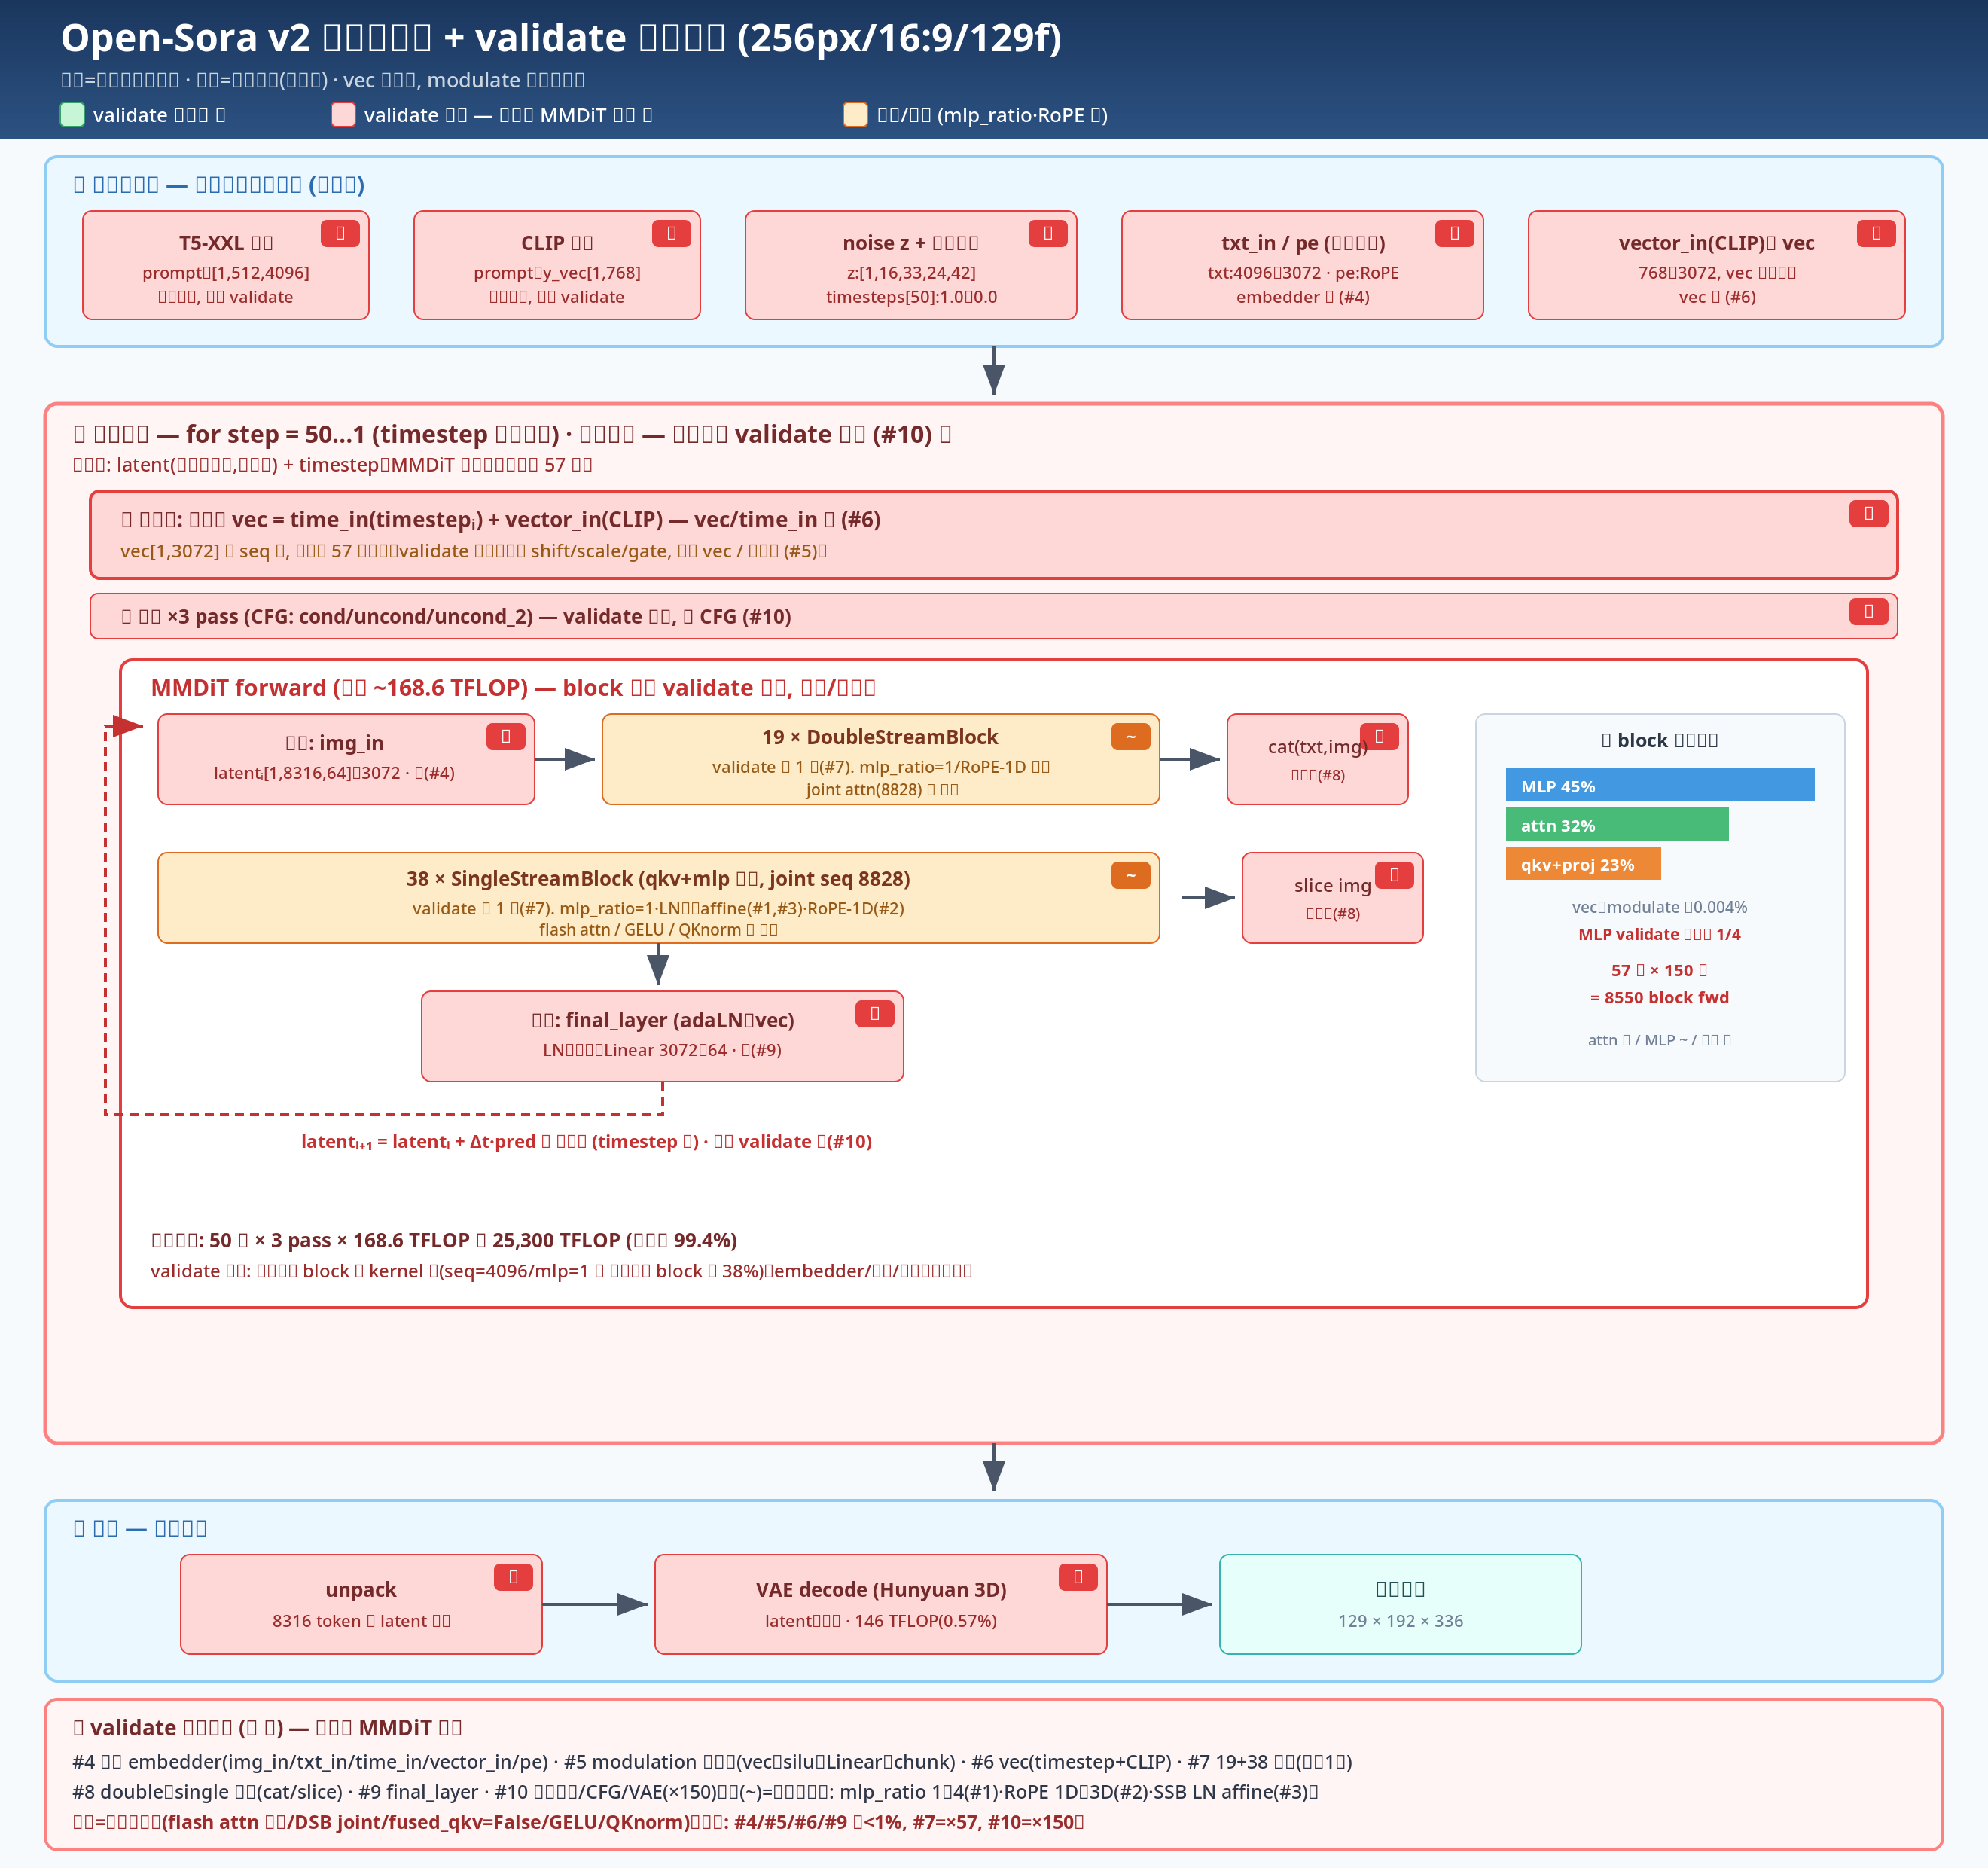
\includegraphics[keepaspectratio,alt={Open-Sora v2 inference flow}]{transactional_emulator/testbench/MMDIT_INFERENCE_FLOW.png}}
\caption{Open-Sora v2 inference flow}
\end{figure}

The MMDiT forward stage is run once per timestep per CFG pass and
operates on a \textbf{joint sequence of 8828 tokens} (8316 image tokens
+ 512 text tokens), with hidden size 3072 across 24 heads. Because it is
executed on the order of 150 times per generation while the encoder and
decoder run only once, it is this stage --- not text encoding or VAE
decoding --- that determines inference cost. The rest of this report
quantifies exactly how dominant it is and drills down to the single
component we set out to accelerate.

\subsubsection{1.2 The two phases that must be
supported}\label{the-two-phases}

Accelerating a deployed model means carrying its \textbf{entire
lifecycle} on the hardware, not only the serving path. The key fact that
simplifies this is that \textbf{the MMDiT is the only part that is
trained}: in Open-Sora's pipeline the \textbf{T5-XXL / CLIP text encoders
and the 3D VAE are pre-trained and frozen} --- they are reused
off-the-shelf and never receive gradients. All training (and all
fine-tuning) happens on the \textbf{MMDiT denoising backbone}. This makes
the MMDiT the single point that determines cost in \emph{both} phases:

\begin{itemize}
\tightlist
\item
  \textbf{Inference} drives the MMDiT \emph{forward} \textasciitilde150×
  per generation (§2 shows it is 99.4\% of generation FLOPs), at low
  precision (MX-E4M3).
\item
  \textbf{Training} drives the MMDiT \emph{backward} (gradient) pass,
  which --- per operator --- costs \textasciitilde2--2.5× the forward
  (§5.2), at high precision (fp32). Because the frozen encoder/VAE
  contribute no backward, training compute is \emph{entirely} MMDiT
  backward.
\end{itemize}

The requirement is therefore: the \emph{same} SingleStreamBlock /
DoubleStreamBlock kernels must lower to PLENA ISA in both a
high-precision backward form (training) and a low-precision forward form
(inference), and one hardware configuration --- matched to an A100's MAC
budget --- must serve both phases.

\subsubsection{1.3 Success criteria}\label{success-criteria}

\begin{enumerate}
\def\labelenumi{\arabic{enumi}.}
\tightlist
\item
  \textbf{Functional.} Both blocks (forward and backward) compile to real
  PLENA \texttt{.isa} and match a reference within the expected rounding
  magnitude of their precision.
\item
  \textbf{Compute-bound.} Memory traffic must be a rounding error vs
  compute at the real Open-Sora geometry in both phases (otherwise a
  compute accelerator is mis-applied).
\item
  \textbf{Competitive at a matched budget.} At a configuration matched to
  one A100's MAC budget on the same 7 nm node, PLENA must deliver a clear
  energy advantage at comparable wall-clock --- for both inference and
  training.
\end{enumerate}

\begin{center}\rule{0.5\linewidth}{0.5pt}\end{center}

\subsection{2. Analysis \& Design}\label{analysis-and-design}

\subsubsection{2.1 Where the compute is --- whole-model
breakdown}\label{whole-model-breakdown}

Counting FLOPs across a full generation (\textasciitilde50 timesteps × 3
CFG passes), MMDiT overwhelmingly dominates:

{\def\LTcaptype{none} % do not increment counter
\begin{longtable}[]{@{}lll@{}}
\toprule\noalign{}
Stage & FLOP & Share \\
\midrule\noalign{}
\endhead
\bottomrule\noalign{}
\endlastfoot
\textbf{MMDiT forward} & \textbf{25,300 TFLOP} & \textbf{99.40\%} \\
VAE decode & 146 TFLOP & 0.58\% \\
T5-XXL / CLIP / embedder / unpack & \textasciitilde5 TFLOP & 0.02\% \\
\end{longtable}
}

One MMDiT forward pass is \textbf{168.6 TFLOP}; multiplied by
\textasciitilde150 invocations this becomes the 25,300 TFLOP that
defines inference cost. \textbf{Accelerating Open-Sora is therefore
equivalent to accelerating the MMDiT forward pass} --- the text encoder
and VAE decoder, run only once each, are together below 0.6\% and not
worth optimizing.

\subsubsection{2.2 Inside one MMDiT pass}\label{inside-one-mmdit-pass}

A single MMDiT pass is a stack of transformer blocks plus a small output
head:

{\def\LTcaptype{none} % do not increment counter
\begin{longtable}[]{@{}
  >{\raggedright\arraybackslash}p{(\linewidth - 8\tabcolsep) * \real{0.2000}}
  >{\raggedright\arraybackslash}p{(\linewidth - 8\tabcolsep) * \real{0.2000}}
  >{\raggedright\arraybackslash}p{(\linewidth - 8\tabcolsep) * \real{0.2000}}
  >{\raggedright\arraybackslash}p{(\linewidth - 8\tabcolsep) * \real{0.2000}}
  >{\raggedright\arraybackslash}p{(\linewidth - 8\tabcolsep) * \real{0.2000}}@{}}
\toprule\noalign{}
\begin{minipage}[b]{\linewidth}\raggedright
Component
\end{minipage} & \begin{minipage}[b]{\linewidth}\raggedright
Count
\end{minipage} & \begin{minipage}[b]{\linewidth}\raggedright
FLOP / block
\end{minipage} & \begin{minipage}[b]{\linewidth}\raggedright
Total / pass
\end{minipage} & \begin{minipage}[b]{\linewidth}\raggedright
Share of pass
\end{minipage} \\
\midrule\noalign{}
\endhead
\bottomrule\noalign{}
\endlastfoot
\textbf{SingleStreamBlock} & \textbf{38} & 2.96 TFLOP & \textbf{112.4
TFLOP} & \textbf{66.6\%} \\
\textbf{DoubleStreamBlock} & 19 & 2.96 TFLOP & 56.2 TFLOP & 33.3\% \\
final\_layer (adaLN + output proj) & 1 & 0.34 TFLOP & 0.34 TFLOP &
0.2\% \\
\textbf{MMDiT pass total} & & & \textbf{168.9 TFLOP} & 100\% \\
\end{longtable}
}

Two facts stand out:

\begin{enumerate}
\def\labelenumi{\arabic{enumi}.}
\tightlist
\item
  \textbf{A SingleStreamBlock and a DoubleStreamBlock cost essentially
  the same per block (\textasciitilde2.96 TFLOP).} The DoubleStreamBlock
  runs two streams (image + text) plus a joint attention; the
  SingleStreamBlock runs one fused stream over the already-concatenated
  joint sequence --- they work out to the same per-block cost.
\item
  \textbf{There are twice as many SingleStreamBlocks (38) as
  DoubleStreamBlocks (19).} So the single-stream layers carry
  \textbf{two-thirds of the entire MMDiT pass}, while the final\_layer
  is negligible (0.2\%).
\end{enumerate}

→ \textbf{The SingleStreamBlock is the heaviest part of MMDiT, and
therefore of the whole model.} This is the block we target for
acceleration; the rest of the report analyzes it in detail. (The
DoubleStreamBlock is structurally two single-stream pipelines plus joint
attention, so the same optimizations carry over; the final\_layer is too
small to matter.)

\subsubsection{2.3 The two blocks we
target}\label{focus-the-single--and-double-stream-blocks}

Together the SingleStreamBlock (66.6\%) and DoubleStreamBlock (33.3\%)
make up \textbf{99.8\% of every MMDiT pass}. The final\_layer is 0.2\%.
\textbf{Our acceleration effort therefore concentrates entirely on these
two block types} --- they are where essentially all the compute lives,
and they share the same set of kernels (norm, modulate, linear, qk-norm,
RoPE, flash attention, gelu, residual), so improvements to one transfer
directly to the other.

The two differ only in topology:

\begin{itemize}
\tightlist
\item
  \textbf{SingleStreamBlock} runs \textbf{one fused stream} over the
  already-concatenated joint sequence (8828 tokens). One norm → modulate
  → q/k/v linear → qk-norm → RoPE → flash attention → fused proj+mlp
  (linear2) → residual.
\item
  \textbf{DoubleStreamBlock} runs \textbf{two independent streams}
  (image + text, separate weights). Each stream does its own
  pre-attention path, then the streams are \textbf{concatenated into a
  single joint sequence for one shared flash attention}, split back
  apart, and each runs its own post-attention path (proj, mlp,
  residual).
\end{itemize}

The heaviest kernel in \textbf{both} blocks is the \textbf{joint flash
attention} --- full bidirectional attention over the long sequence (no
causal mask, no KV cache), which is why it dominates the matmul and
vector work in either topology.

\subsubsection{2.3.1 SingleStreamBlock
structure}\label{singlestreamblock-structure}

\begin{figure}
\centering
\pandocbounded{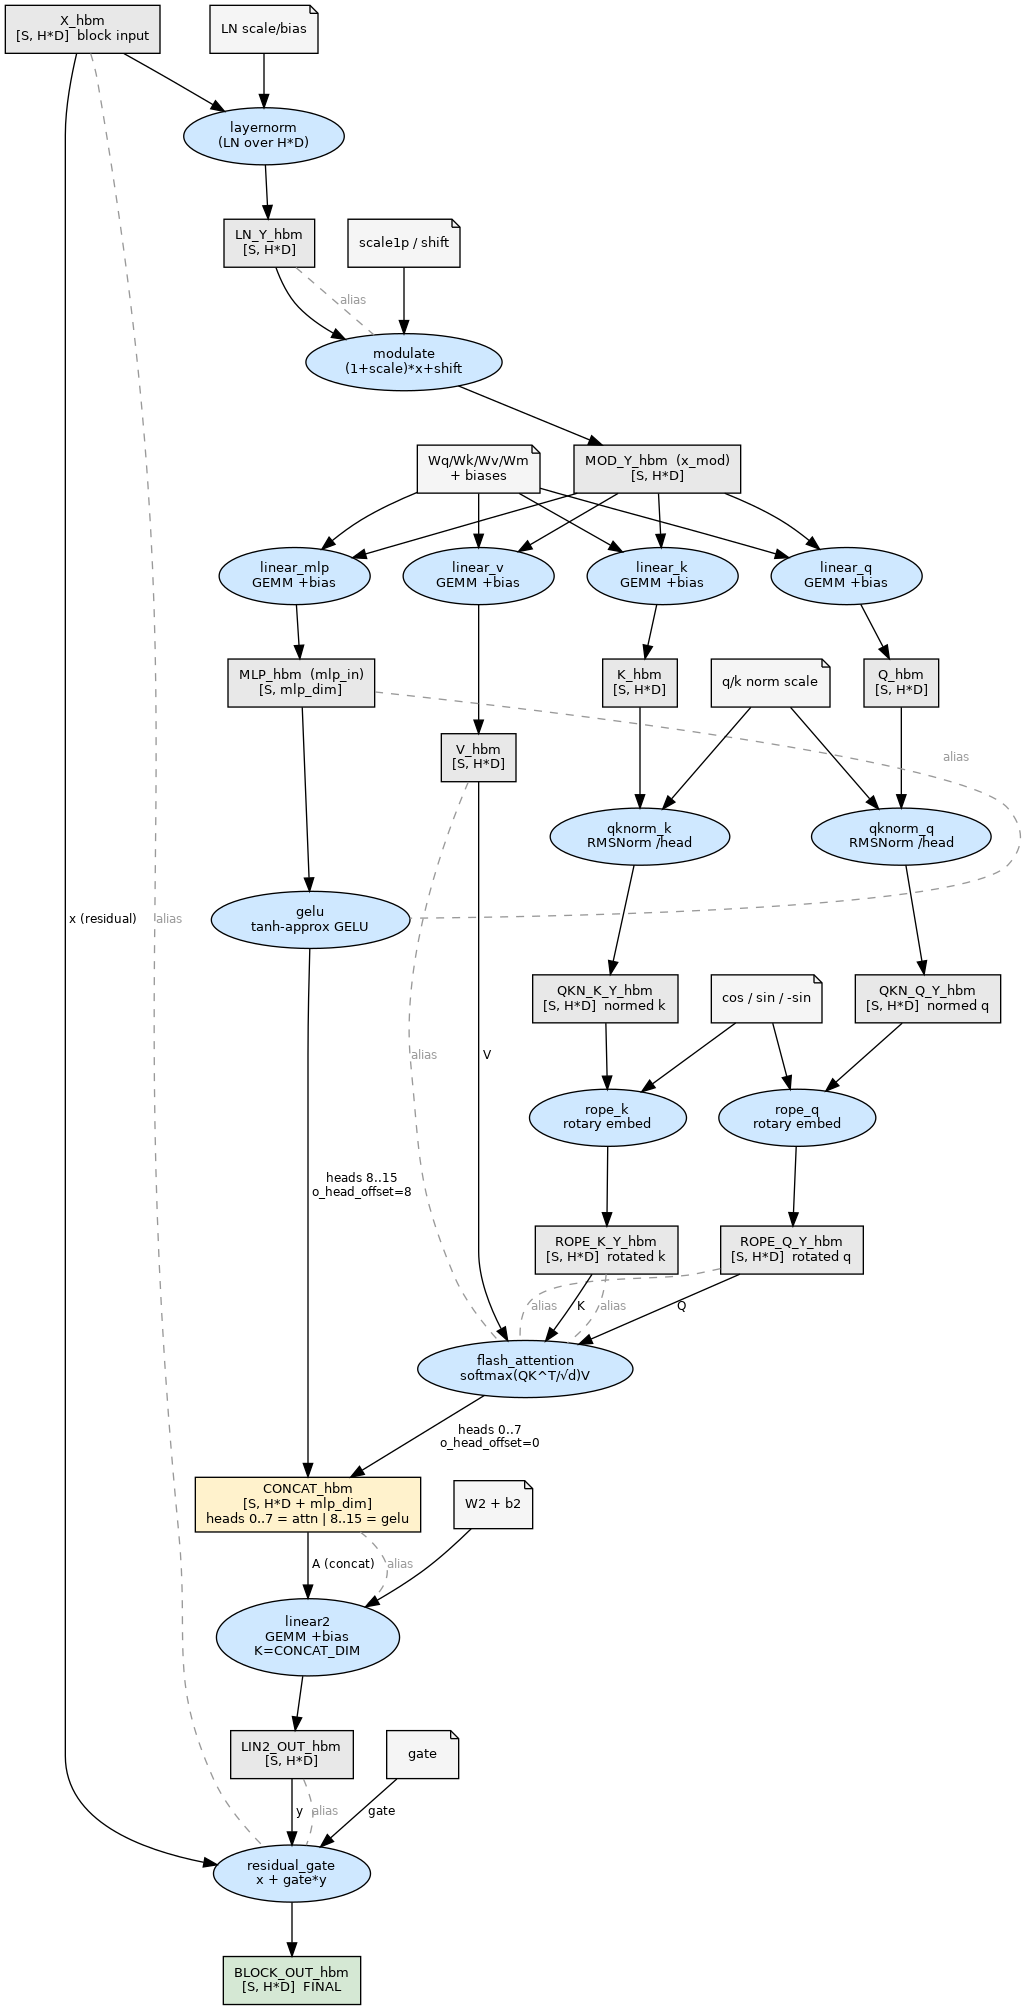
\includegraphics[keepaspectratio,alt={SingleStreamBlock data-flow graph}]{transactional_emulator/testbench/single_stream_block_graph.png}}
\caption{SingleStreamBlock data-flow graph}
\end{figure}

\subsubsection{2.3.2 DoubleStreamBlock
structure}\label{doublestreamblock-structure}

\begin{figure}
\centering
\pandocbounded{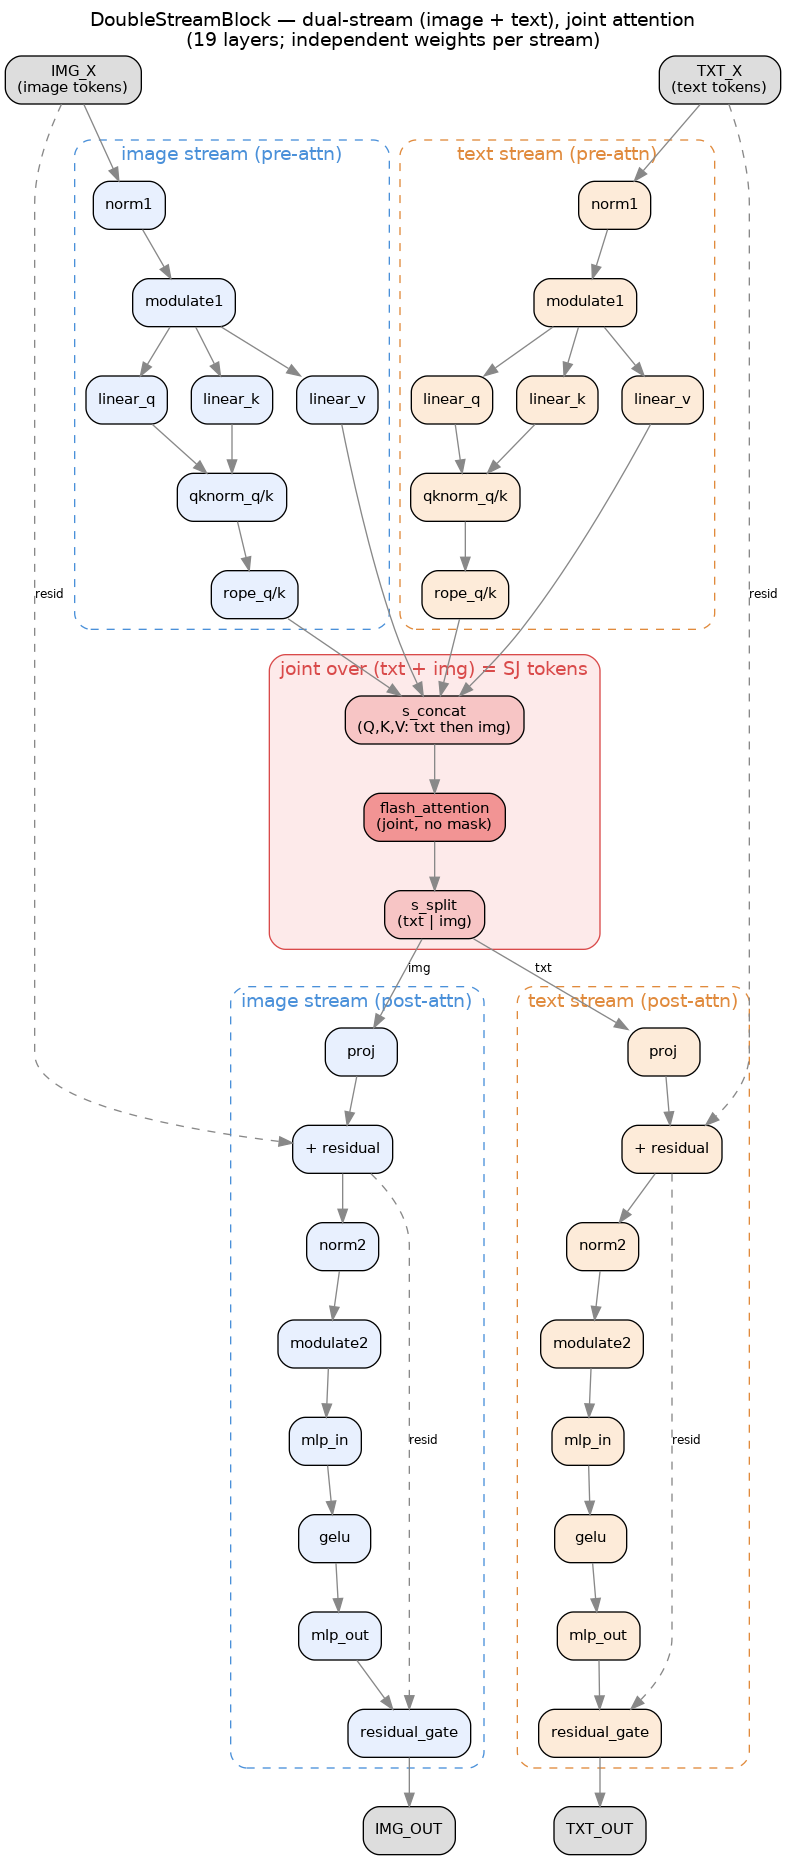
\includegraphics[keepaspectratio,alt={DoubleStreamBlock data-flow graph}]{transactional_emulator/testbench/double_stream_block_graph.png}}
\caption{DoubleStreamBlock data-flow graph}
\end{figure}

\subsubsection{2.4 Precision design --- low (MX-E4M3) vs high (fp32),
a tunable knob}\label{precision-design}

The same blocks run at \textbf{two different precisions} depending on
phase, and precision is modelled as an explicit knob that scales both the
power and the memory traffic:

\begin{itemize}
\tightlist
\item
  \textbf{Inference (forward) → MX-E4M3 (low precision, 1×).} The denoising
  loop is the latency- and energy-critical path (it runs \textasciitilde150×
  per generation), so the forward runs at low precision. All HBM tensors
  are MX-E4M3 (8-bit element + E8M0 block scale), trading a small amount of
  accuracy for the lowest-energy operating point — this is the 1× baseline
  for the power model.
\item
  \textbf{Training (backward + optimizer) → fp32 (high precision, 2×).}
  Gradients span a wide dynamic range and low-precision accumulation
  degrades convergence, so training keeps fp32 (32-bit) elements. The
  wider datapath roughly \textbf{doubles the per-unit power} (MAC, vector
  lane, and SRAM all ×2 vs the FP8/MX baseline) and doubles the HBM bytes
  per element.
\end{itemize}

\textbf{What precision does and does not change.} Precision is
\emph{cycle-invariant} but \emph{not} energy-invariant. The cycle count
(and hence latency) is fixed by the systolic-array geometry (BLEN × MLEN)
and the operation count — a fp32 GEMM takes the same cycles as an FP8 GEMM
on the same array. But the datatype scales the power on \textbf{two
separate legs}, anchored to the \textbf{FP16 baseline} (MAC = 1 mW, vector
lane = 0.5 mW, SRAM = 0.055 pJ/bit):

\begin{itemize}
\tightlist
\item
  \textbf{MCU (matmul)} scales with the \emph{accumulation} precision. FP8
  multiplies accumulate into FP16, so the MAC array stays at the FP16 power
  level — \textbf{FP8 MCU = 1×, not halved}; only fp32 accumulation makes
  it 2×.
\item
  \textbf{Vector unit + both SRAMs} scale with the \emph{element bit-width}:
  FP8 = 0.5×, FP16 = 1×, fp32 = 2×. The HBM byte count (8 / 16 / 32-bit)
  tracks this and scales memory time.
\end{itemize}

So inference (MX-E4M3: MCU 1×, vector/SRAM 0.5×) is the low-energy point,
and training (fp32: everything 2×) is the high-energy point — same cycles,
different energy. The energy tool exposes \texttt{-{}-precision} as a
first-class option (\texttt{mx\_e4m3 / fp8 / fp16 / bf16 / fp32}).

\subsubsection{2.5 Fine-tuning --- the bridge between the
phases}\label{fine-tuning-bridge}

Between high-precision training and low-precision inference sits
\textbf{fine-tuning}, the mechanism that makes a model trained at fp32
run correctly at MX-E4M3:

\begin{itemize}
\tightlist
\item
  \textbf{Why it is needed.} A model trained at fp32 and then naively
  cast to MX-E4M3 loses accuracy at the activation/weight quantization
  boundaries (the long-tail values in attention scores and MLP
  activations are the most sensitive). Fine-tuning closes this gap.
\item
  \textbf{How it works.} Either \emph{post-training calibration} (collect
  activation statistics on a calibration set, choose per-block MX scales,
  no weight update) or \emph{quantization-aware fine-tuning} (a short
  fp32 backward pass with a simulated MX-E4M3 forward in the loop, so the
  weights learn to be robust to the quantiser). Both reuse exactly the
  training-phase backward kernels analysed in §5.2 --- fine-tuning is a
  \textbf{bounded number of training steps}, not a new kernel set.
\item
  \textbf{Cost positioning.} Because it reuses the training backward and
  runs for only a small number of steps, fine-tuning's cost is dominated
  by the same matmul-bound backward profile; it is treated here
  qualitatively as the connective stage, not measured separately.
\end{itemize}

\begin{center}\rule{0.5\linewidth}{0.5pt}\end{center}

\subsection{3. Implementation}\label{implementation}

\subsubsection{3.1 GPU reference implementation: TileLang vs.~PyTorch on
A100}\label{gpu-baseline-tilelang-vs.-pytorch-on-a100}

We compiled both blocks at the \textbf{real Open-Sora v2 dimensions}
(hidden 3072, 24 heads, mlp\_ratio = 4), padding the sequence dimensions
to multiples of 1024:

\begin{itemize}
\tightlist
\item
  \textbf{SingleStreamBlock} --- joint sequence S = 9216 (8828 → padded
  to 9216).
\item
  \textbf{DoubleStreamBlock} --- image stream 9216 (8316 → 9216), text
  stream 1024 (512 → 1024), joint = 10240.
\end{itemize}

Both sides are run at \textbf{batch size = 4}. This is required to keep
the A100 fully utilized: in the TileLang schedule, every SM must be
given work, which means the launch grid must expose at least as many
blocks as there are SMs (\(\geq\) 96). A single batch does not produce enough
blocks to cover all SMs, so we use a batch of 4, which pushes the block
count past the SM threshold and saturates the GPU. This batch-4 shape is
the configuration used for all comparisons below.

We first establish the \textbf{GPU baseline} on an \textbf{NVIDIA
A100-80GB} (bf16, batch = 4), measuring our own TileLang implementation
of each block against the standard PyTorch + SDPA reference. Both run on
the same A100; this isolates the TileLang kernel quality on a GPU before
we move the design onto PLENA. Latency, average power, and energy per
block are reported below.

\textbf{Correctness.} Both TileLang implementations match the PyTorch
reference to a max-abs-diff of \textbf{0.0156} --- the expected bf16
rounding magnitude, and identical to the batch-1 result, confirming that
the batch-4 extension introduces no error.

\textbf{SSB} (\texttt{bench\_ssb.py})

{\def\LTcaptype{none} % do not increment counter
\begin{longtable}[]{@{}llll@{}}
\toprule\noalign{}
Impl. & Latency & Avg power & Energy / block \\
\midrule\noalign{}
\endhead
\bottomrule\noalign{}
\endlastfoot
PyTorch + SDPA & \textbf{73.4 ms} & 393 W & \textbf{28.9 J} \\
TileLang & 85.1 ms & 388 W & 33.0 J \\
Ratio & 0.86× (slower) & slightly lower & 0.87× \\
\end{longtable}
}

\textbf{DSB} (\texttt{bench\_dsb.py})

{\def\LTcaptype{none} % do not increment counter
\begin{longtable}[]{@{}llll@{}}
\toprule\noalign{}
Impl. & Latency & Avg power & Energy / block \\
\midrule\noalign{}
\endhead
\bottomrule\noalign{}
\endlastfoot
PyTorch + SDPA & \textbf{87.4 ms} & 391 W & \textbf{34.2 J} \\
TileLang & 101.1 ms & 440 W & 44.5 J \\
Ratio & 0.86× (slower) & higher & 0.77× \\
\end{longtable}
}

\textbf{Reading the result.} On the A100, our TileLang kernels land at
\textbf{0.86×} the speed of PyTorch + SDPA for both blocks, at
comparable (SSB) or somewhat higher (DSB) power. This sets the GPU
reference point: a hand-written TileLang schedule on the A100 is within
\textasciitilde15\% of the vendor library. The next sections move this
same workload onto PLENA and analyze where its cycles and energy go.

\begin{center}\rule{0.5\linewidth}{0.5pt}\end{center}

\subsubsection{3.2 GPU-equivalent compute: choosing the PLENA
configuration}\label{gpu-equivalent-compute-choosing-the-plena-configuration}

The A100 comparison in §3.1 is only fair if the two chips are matched on
raw matrix-compute resources. This section counts the
multiply-accumulate (MAC) units on each side and uses that count to
\textbf{fix the PLENA hardware configuration} for all measurements in
this report.

\paragraph{3.2.1 A100 MAC count}\label{a100-mac-count}

The A100 is built from a hierarchy of multiply-accumulate arrays:

\begin{itemize}
\tightlist
\item
  \textbf{108 SMs}, each with \textbf{4 Tensor Cores} → \textbf{432
  Tensor Cores} total.
\item
  Each Tensor Core performs \textbf{256 MACs per cycle} for BF16/FP16.
\end{itemize}

\[\text{A100 MACs} = 108 \times 4 \times 256 = 110{,}592 \text{ MAC}\]

We cross-check this count against the published spec. Counting one MAC
as 2 FLOPs (NVIDIA's convention) at the 1.41 GHz boost clock:

\[110{,}592 \times 2 \times 1.41\,\text{GHz} = 312\ \text{TFLOPS (BF16)}\]

which matches NVIDIA's published \textbf{312 TFLOPS} BF16/FP16 Tensor
Core peak exactly --- confirming the 256-MAC-per-Tensor-Core count.

\paragraph{3.2.2 PLENA per-device MAC count and the multi-device
match}\label{plena-per-device-mac-count-and-the-multi-device-match}

A single PLENA device is a systolic array of dimension \textbf{BLEN ×
MLEN}, with MLEN fixed at 1024. We run each device at \textbf{BLEN = 8},
so one device holds

\[\text{PLENA MACs (per device)} = 8 \times 1024 = 8{,}192 \text{ MAC}\]

This is deliberately small --- one PLENA device has only
\textasciitilde7\% of the A100's MAC budget. Rather than grow a single
die to A100 scale, PLENA matches the GPU by \textbf{replicating small
devices and running them in parallel}. To reach the A100's MAC budget we
deploy \textbf{12 devices}:

\[12 \times 8{,}192 = 98{,}304 \text{ MAC} \;\approx\; 0.89\times \text{ the A100's } 110{,}592\]

Twelve BLEN-8 devices therefore put PLENA in the same hardware class as
one A100 (within \textasciitilde11\% on MAC count), while each device
stays small, low-power, and high-yield. This 12-device, BLEN-8
configuration is the deployment behind §5--§6; the per-device analytic
numbers come from \texttt{plena\_settings.toml} (BLEN = 8) and the
per-block reports.

At BLEN = 8 and the 1.0 GHz clock, one device's peak BF16 throughput is
\(8{,}192 \times 2 \times 1.0\,\text{GHz} = 16.4\) TFLOPS; twelve
devices give \textbf{197 TFLOPS} aggregate.

\paragraph{3.2.3 Side-by-side}\label{side-by-side}

{\def\LTcaptype{none} % do not increment counter
\begin{longtable}[]{@{}
  >{\raggedright\arraybackslash}p{(\linewidth - 6\tabcolsep) * \real{0.2500}}
  >{\raggedright\arraybackslash}p{(\linewidth - 6\tabcolsep) * \real{0.2500}}
  >{\raggedright\arraybackslash}p{(\linewidth - 6\tabcolsep) * \real{0.2500}}
  >{\raggedright\arraybackslash}p{(\linewidth - 6\tabcolsep) * \real{0.2500}}@{}}
\toprule\noalign{}
\begin{minipage}[b]{\linewidth}\raggedright
\end{minipage} & \begin{minipage}[b]{\linewidth}\raggedright
NVIDIA A100
\end{minipage} & \begin{minipage}[b]{\linewidth}\raggedright
PLENA (12 × BLEN-8 devices)
\end{minipage} & \begin{minipage}[b]{\linewidth}\raggedright
Ratio (PLENA / A100)
\end{minipage} \\
\midrule\noalign{}
\endhead
\bottomrule\noalign{}
\endlastfoot
MAC array & 432 TC × 256 = \textbf{110,592 MAC} & 12 × (8 × 1024) =
\textbf{98,304 MAC} & \textbf{0.89×} \\
Clock & 1.41 GHz & 1.0 GHz & 0.71× \\
\textbf{Peak BF16} & \textbf{312 TFLOPS} & \textbf{197 TFLOPS} &
\textbf{0.63×} \\
\end{longtable}
}

The 12-device PLENA deployment carries \textbf{\textasciitilde11\% fewer
MAC units} than an A100 and runs at a \textbf{lower clock (0.71×)}, for
an aggregate peak BF16 throughput of \textbf{0.63×} the A100's. Both are
on a \textbf{7 nm node} (the A100 is NVIDIA's Ampere GA100 on TSMC N7),
so the comparison reflects architecture and dataflow, not a process gap.
§5 places PLENA's per-block latency and energy at this 12-device
configuration directly against the A100 baseline of §3.1.

\subsubsection{3.3 PLENA ISA implementation --- both phases compiled, not
estimated}\label{isa-implementation-both-phases}

Every kernel --- forward (inference) and backward (training) --- was
\textbf{compiled end-to-end to real PLENA \texttt{.isa}} and measured by
the energy tool; nothing is estimated from FLOP counts:

\begin{itemize}
\tightlist
\item
  \textbf{Inference (forward).} All blocks compiled at the real
  dimensions (mlp\_ratio = 4), HBM tensors in MX-E4M3.
\item
  \textbf{Training (backward).} All \textbf{19 SSB backward kernels}
  (\texttt{managerbuild\_bwd\_chain/ir}) and all \textbf{47 DSB backward
  kernels} (\texttt{managerbuild\_bwd\_double/ir}) compiled to ISA; every
  kernel's gradient is the exact analytic backward of its forward
  operator. HBM in fp32.
\end{itemize}

The cycle/energy methodology is identical across both phases:

\begin{itemize}
\tightlist
\item
  \textbf{Cycle formula:} George performance customISA (pipelined column;
  \(M_{BMM} = \text{BLEN}\cdot(\text{MLEN}/\text{BLEN})^2 = 131{,}072\),
  \(M_{MM} = \text{BLEN} = 8\)). 1 cycle = 1 ns at 1.0 GHz.
\item
  \textbf{compute = matmul + vector + scalar\_fp} (scalar\_int / ldst /
  control NOT counted), measured by
  \texttt{tools/power/plena\_isa\_energy.py}.
\item
  \textbf{Power model (bottom-up, 7 nm, BF16→FP32):} MAC = 1 mW, vector
  lane = 0.5 mW, SRAM = 0.055 pJ/bit. At BLEN = 8: MCU = 8.2 W, vector =
  0.512 W, each SRAM = 0.901 W.
\end{itemize}

\paragraph{Backward-pass lowering notes (training).}\label{bwd-lowering}

The backward kernels reuse the forward operator set with
gradient-specific GEMMs. Two PLENA-specific points:

\begin{itemize}
\tightlist
\item
  \textbf{Transpose-A.} Attention \(dQ = dS\cdot K\) and every linear
  \(dW = dY^{\top}\!\cdot X\) need a \emph{non-transposed activation} as
  the VRAM (A) operand, but the MRAM transpose unit (M\_TMM) only
  transposes the B operand. We therefore add a dedicated transpose
  \textbf{buffer} that corner-turns the activation into the MRAM, matching
  the MRAM datapath, so the GEMM contracts the correct axis and is
  mathematically exact. The corner-turn is \textasciitilde MLEN cycles of
  pure data movement (negligible energy).
\item
  \textbf{Everything else lowers cleanly.} Attention
  \(S^{\top}\)/\(dP^{\top}\)/\(dV\)/\(dK\), rope, and linear \(dW\) use
  transpose-B; linear \(dX = dY\cdot W\) uses a plain matmul (W stored
  \([N,K]\), hand-accumulated N-partials) --- mathematically exact, no
  transpose. All vector backward kernels (gelu\('\), RMS/LayerNorm
  Jacobians) are exact and stay off the matmul critical path.
\end{itemize}

\subsubsection{3.4 Device allocation --- splitting one kernel across
devices}\label{device-allocation}

The multi-device scaling used throughout §5--§6 (one block split across N
PLENA devices, latency ÷ N at fixed energy) needs almost no machinery,
because it rides the \textbf{multi-thread structure that TileLang and the
GPU programming model already expose}. A TileLang kernel launches a grid of
thread-blocks indexed by \texttt{blockIdx}; every block is an independent
unit of work over a tile of the problem (a sequence chunk, a head group).
PLENA inherits this: the compiler already lowers the kernel into per-block
work, so distributing it is just deciding \emph{which device runs which
block}.

The whole mechanism is one step at the \textbf{end of the mid-IR}: the
multi-threaded \texttt{blockIdx} is \textbf{instantiated per device} — each
device is handed a contiguous slice of the block range. With \(B\) blocks
and \(N\) devices, device \(d\) runs blocks \([d\cdot B/N,\ (d{+}1)\cdot
B/N)\). Nothing in the kernel body changes; the blocks were already
independent, so partitioning them across devices is sound by construction
and the per-device ISA is identical.

\textbf{When there are fewer devices than blocks}, the surplus blocks are
handled by a \textbf{block-id loop}: a device that owns more than one block
simply iterates its assigned block ids serially (the same loop the
single-device build already runs over the full range, now bounded to the
device's slice). So the two regimes are the same code path —
\(N \geq B\) gives one block per device (latency ÷ N), and \(N < B\) loops
\(\lceil B/N\rceil\) blocks per device. This is why the device sweep in
§5--§6 is clean linear scaling: it is literally the GPU's own block-parallel
execution model, mapped onto N PLENA devices at the mid-IR boundary, with a
loop covering the remainder.

\begin{center}\rule{0.5\linewidth}{0.5pt}\end{center}

\subsection{4. Test Plan and
Verification}\label{test-plan-and-verification}

\subsubsection{4.1 Functional correctness --- inference
(forward)}\label{correctness-inference}

Both TileLang block implementations match the PyTorch + SDPA reference to
a \textbf{max-abs-diff of 0.0156} (§3.1) --- the expected bf16 rounding
magnitude, identical to the batch-1 result, confirming the batch-4
extension introduces no error.

\subsubsection{4.2 Functional correctness --- training
(backward)}\label{correctness-training}

Every backward kernel is the \textbf{exact analytic backward} of its
forward operator and is compiled end-to-end (not estimated). The
backward/forward matmul ratios are verified against the structural rules:

{\def\LTcaptype{none} % do not increment counter
\begin{longtable}[]{@{}
  >{\raggedright\arraybackslash}p{(\linewidth - 4\tabcolsep) * \real{0.2600}}
  >{\raggedright\arraybackslash}p{(\linewidth - 4\tabcolsep) * \real{0.2400}}
  >{\raggedright\arraybackslash}p{(\linewidth - 4\tabcolsep) * \real{0.5000}}@{}}
\toprule\noalign{}
\begin{minipage}[b]{\linewidth}\raggedright
Operator class
\end{minipage} & \begin{minipage}[b]{\linewidth}\raggedright
bwd matmul vs fwd
\end{minipage} & \begin{minipage}[b]{\linewidth}\raggedright
why
\end{minipage} \\
\midrule\noalign{}
\endhead
\bottomrule\noalign{}
\endlastfoot
\textbf{Linear (+bias)} ×5 & \textbf{2.0×} & fwd 1 GEMM (\(X\!\cdot\!W^{\top}\)); bwd 2
(\(dX = dY\!\cdot\!W\), \(dW = dY^{\top}\!\cdot\!X\)) \\
\textbf{Attention} & \textbf{2.5×} (measured) & fwd 2 GEMM; bwd 5 (\(S^{\top}\),
\(dP^{\top}\), dV, dK, dQ) \\
\textbf{RoPE} ×2 & \textbf{1.0×} & P is a symmetric permutation (\(P = P^{\top} = P^{-1}\)) \\
\textbf{GELU} & matmul 0 & \(dX = dY\!\cdot\!\mathrm{gelu}'(x)\): vector \textasciitilde3×
fwd \\
\textbf{RMS/LayerNorm} & matmul 0 & dX needs the normalise Jacobian:
\textasciitilde2× fwd vector \\
\textbf{affine} & matmul 0 & \(dX = dY\!\cdot\!\text{factor}\): \textasciitilde1× fwd
vector \\
\end{longtable}
}

The two transpose-A GEMMs (attention dQ, linear dW) use the dedicated
transpose buffer (§3.3) to corner-turn the activation into the MRAM, so
they contract the correct axis and are mathematically exact.

\subsubsection{4.3 Memory verification --- the workload is compute-bound
(both phases)}\label{memory-and-hbm-bandwidth}

A latency comparison only holds if the accelerator is genuinely
\textbf{compute-bound} and not secretly limited by memory traffic. This
section shows that the Open-Sora blocks are firmly compute-bound on
PLENA, with large headroom on HBM bandwidth.

\paragraph{4.3.1 Bandwidth available}\label{bandwidth-available}

PLENA moves data between HBM and the on-chip SRAMs over two DMA ports
--- a matrix port and a vector port --- each one MLEN-wide (and
VLEN-wide) per cycle:

\[\text{per-port BW} = 1024\ \text{B/cyc} \times 1.0\ \text{GHz} = 1024\ \text{GB/s}, \qquad \text{total} \approx 2{,}048\ \text{GB/s}\]

This is comparable to the A100-80GB's HBM2e bandwidth (\textbf{2,039
GB/s} SXM / 1,940 GB/s PCIe), so the two are in the same
memory-bandwidth class --- the comparison is not biased by giving PLENA
an unrealistic memory subsystem.

\paragraph{4.3.2 Traffic and time per block (batch =
4)}\label{traffic-and-time-per-block-batch-4}

All HBM tensors are stored in MX format (E4M3 element + E8M0 block
scale, block = 8), so the byte count includes a 1.25× scale overhead.
Dividing the per-block HBM traffic by the available bandwidth gives the
memory time:

{\def\LTcaptype{none} % do not increment counter
\begin{longtable}[]{@{}
  >{\raggedright\arraybackslash}p{(\linewidth - 8\tabcolsep) * \real{0.2000}}
  >{\raggedright\arraybackslash}p{(\linewidth - 8\tabcolsep) * \real{0.2000}}
  >{\raggedright\arraybackslash}p{(\linewidth - 8\tabcolsep) * \real{0.2000}}
  >{\raggedright\arraybackslash}p{(\linewidth - 8\tabcolsep) * \real{0.2000}}
  >{\raggedright\arraybackslash}p{(\linewidth - 8\tabcolsep) * \real{0.2000}}@{}}
\toprule\noalign{}
\begin{minipage}[b]{\linewidth}\raggedright
Block
\end{minipage} & \begin{minipage}[b]{\linewidth}\raggedright
HBM traffic / block
\end{minipage} & \begin{minipage}[b]{\linewidth}\raggedright
Memory time
\end{minipage} & \begin{minipage}[b]{\linewidth}\raggedright
Compute time (1 device)
\end{minipage} & \begin{minipage}[b]{\linewidth}\raggedright
Memory / compute
\end{minipage} \\
\midrule\noalign{}
\endhead
\bottomrule\noalign{}
\endlastfoot
SSB & 356 MB & 0.35 ms & 1077.7 ms & \textbf{0.03\%} \\
DSB & 509 MB & 0.50 ms & 1257.7 ms & \textbf{0.04\%} \\
\end{longtable}
}

\paragraph{4.3.3 Worst-case HBM contention (one block split across 12
devices)}\label{worst-case-hbm-contention-one-block-split-across-12-devices}

In the 12-device deployment a single block is \textbf{split across the
12 devices by TileLang}, not replicated. The total HBM traffic is
therefore \textbf{fixed --- it is exactly one block's worth (356 MB SSB
/ 509 MB DSB)} --- just partitioned so each device fetches its 1/12
share. What changes is that all 12 devices want to read from the shared
HBM at the same time, each at its full port bandwidth, so the accesses
must queue.

We take the most pessimistic queuing model: a single shared HBM pool of
\textbf{2,039 GB/s}, with every device's traffic \textbf{fully
serialized through it} (round-robin, one device served at a time --- no
parallel HBM access at all). The HBM is then busy for

\[t_\text{HBM busy} = \frac{\text{block traffic}}{2{,}039\ \text{GB/s}}\]

and we compare that against the per-block latency at the 12-device
configuration (compute / 12):

{\def\LTcaptype{none} % do not increment counter
\begin{longtable}[]{@{}
  >{\raggedright\arraybackslash}p{(\linewidth - 8\tabcolsep) * \real{0.2000}}
  >{\raggedright\arraybackslash}p{(\linewidth - 8\tabcolsep) * \real{0.2000}}
  >{\raggedright\arraybackslash}p{(\linewidth - 8\tabcolsep) * \real{0.2000}}
  >{\raggedright\arraybackslash}p{(\linewidth - 8\tabcolsep) * \real{0.2000}}
  >{\raggedright\arraybackslash}p{(\linewidth - 8\tabcolsep) * \real{0.2000}}@{}}
\toprule\noalign{}
\begin{minipage}[b]{\linewidth}\raggedright
Block
\end{minipage} & \begin{minipage}[b]{\linewidth}\raggedright
Total traffic (fixed)
\end{minipage} & \begin{minipage}[b]{\linewidth}\raggedright
HBM busy time (fully serialized @ 2,039 GB/s)
\end{minipage} & \begin{minipage}[b]{\linewidth}\raggedright
Block latency (12 devices)
\end{minipage} & \begin{minipage}[b]{\linewidth}\raggedright
\textbf{HBM duty cycle}
\end{minipage} \\
\midrule\noalign{}
\endhead
\bottomrule\noalign{}
\endlastfoot
SSB & 356 MB & 0.17 ms & 89.81 ms & \textbf{0.19\%} \\
DSB & 509 MB & 0.24 ms & 104.81 ms & \textbf{0.23\%} \\
\end{longtable}
}

Even in this worst case --- all HBM accesses pushed through one 2,039
GB/s pipe with zero concurrency --- the shared HBM is \textbf{busy only
\textasciitilde0.2\% of the wall-clock}, leaving
\textbf{\textasciitilde430--530× headroom}. Because the work is
\emph{split} rather than replicated, the total bytes to move never grow
with device count; queuing only reorders these few hundred MB in time,
and there is far more than enough bandwidth to drain the queue long
before the compute needs the data. HBM bandwidth is sufficient under the
most pessimistic shared-pool, fully-serialized assumption.

\paragraph{4.3.4 Implication}\label{implication}

Memory time is \textbf{three to four orders of magnitude smaller than
compute time} for both blocks. Under the overlapped
\texttt{total\ =\ max(compute,\ memory)} model every kernel is
compute-bound, and the DMA traffic hides completely behind computation.
Two consequences:

\begin{itemize}
\tightlist
\item
  The latency and energy numbers in §5 are governed entirely by the
  matrix/vector compute, not by memory --- the HBM subsystem is never
  the bottleneck at this geometry.
\item
  Device-level scaling (§5) does not stress aggregate bandwidth: as
  §4.3.3 shows, even 12 devices in parallel demand under 5 GB/s,
  \textasciitilde0.2\% of one A100's HBM bandwidth.
\end{itemize}

This is expected for the Open-Sora MMDiT blocks --- they are dense,
high-arithmetic-intensity GEMMs and attention over a long sequence,
where each byte fetched from HBM is reused across many MAC operations.
The workload is compute-bound by construction, which is exactly the
regime a systolic matrix core is built to exploit.

\subsubsection{4.4 Quantization accuracy --- the verification
methodology}\label{quant-accuracy-methodology}

Accuracy is the hardest of the three quantities to pin down (latency and
energy fall straight out of the ISA analysis of §3.3 / §5), and it is
verified through a deliberate four-stage chain that lets us trust a
\emph{GPU} accuracy measurement as a proxy for the PLENA hardware:

\begin{enumerate}
\def\labelenumi{\arabic{enumi}.}
\tightlist
\item
  \textbf{Simulator anchors numerical correctness.} The PLENA transactional
  simulator does not model the pipeline in enough detail to give latency,
  but it \emph{is} bit-faithful on the arithmetic. We run a single layer /
  structure on the simulator and confirm its output matches the
  quantized golden reference --- this validates that our quantization
  convention (per-op datatypes, MX / FP8 rounding, accumulation order)
  matches what the hardware actually computes.
\item
  \textbf{Move the quantization to GPU.} The simulator is far too slow to
  run a whole model. Once a layer is confirmed to satisfy
  ``simulator output == quantized golden'', we reproduce the \emph{same}
  quantization on the GPU (identical data types, the same per-operator
  rounding). The two agree numerically by construction, so the GPU now
  stands in for the hardware on accuracy.
\item
  \textbf{Run the whole model on GPU.} With every operator's quantization
  matched, we run the full MMDiT on the GPU and measure accuracy (cosine /
  NRMSE vs the FP32 reference) and, crucially, \textbf{how the
  quantization error propagates} through the model.
\item
  \textbf{Latency / energy come from the ISA.} Orthogonally, the same
  kernels are compiled to PLENA ISA and analyzed (§3.3, §5) for cycles and
  energy. Datatype is \emph{cycle-invariant} (latency unchanged) but
  scales the energy: per-unit power ×1 at low precision / ×2 at high
  precision, plus the HBM byte count (§2.4). The accuracy measurement and
  the latency/energy model share no path.
\end{enumerate}

This is why the accuracy numbers below are measured on an A100 (bf16
storage, fp32 accumulation, FP8 round-trip where stated) yet describe the
PLENA deployment: the GPU is running the hardware-matched quantization.

\paragraph{4.4.1 Forward numerical correctness (TileLang vs
PyTorch+SDPA)}\label{fwd-numeric}

Both block implementations match the PyTorch + SDPA reference at the real
Open-Sora dimensions:

{\def\LTcaptype{none}
\begin{longtable}[]{@{}llll@{}}
\toprule\noalign{}
& cosine & abs-max & rel p99 \\
\midrule\noalign{}
\endhead
\bottomrule\noalign{}
\endlastfoot
SSB & \textbf{1.000000} & 0.0156 & 0.0079 \\
DSB (img) & \textbf{0.999999} & 0.0156 & 0.0108 \\
DSB (txt) & \textbf{0.999999} & 0.0156 & 0.0111 \\
\end{longtable}
}

The abs-max of 0.0156 is the bf16 quantization floor, not an algorithmic
error (it is identical across all three and matches the bf16 ULP at this
magnitude).

\paragraph{4.4.2 FP8 quantization --- ``erasing'' the quantization
loss}\label{fp8-quant}

On the \emph{real} Open-Sora-v2 weights, we quantize to FP8 (E4M3) and
measure the output's cosine / NRMSE against the FP32 teacher. Two
granularities, both at the real dimensions:

{\def\LTcaptype{none}
\begin{longtable}[]{@{}
  >{\raggedright\arraybackslash}p{(\linewidth - 6\tabcolsep) * \real{0.3400}}
  >{\raggedright\arraybackslash}p{(\linewidth - 6\tabcolsep) * \real{0.3000}}
  >{\raggedright\arraybackslash}p{(\linewidth - 6\tabcolsep) * \real{0.1800}}
  >{\raggedright\arraybackslash}p{(\linewidth - 6\tabcolsep) * \real{0.1800}}@{}}
\toprule\noalign{}
\begin{minipage}[b]{\linewidth}\raggedright
Scheme
\end{minipage} & \begin{minipage}[b]{\linewidth}\raggedright
quantized
\end{minipage} & \begin{minipage}[b]{\linewidth}\raggedright
PTQ cos
\end{minipage} & \begin{minipage}[b]{\linewidth}\raggedright
QAT cos
\end{minipage} \\
\midrule\noalign{}
\endhead
\bottomrule\noalign{}
\endlastfoot
\textbf{W8A16} (weight-only) & weights, per-output-channel scale &
\textbf{0.99973} & \textbf{0.99976} \\
\textbf{W8A8} (weight + activation) & + per-token dynamic activation scale,
both GEMM operands FP8 & \textbf{0.99944} & \textbf{0.99948} \\
\end{longtable}
}

Three findings:

\begin{itemize}
\tightlist
\item
  \textbf{8-bit (E4M3) is a near-lossless safe zone.} With per-output-channel
  scale calibration, plain PTQ already reaches cos \textbf{0.9997}
  (weight-only) / \textbf{0.9994} (W8A8) --- no fine-tuning needed.
\item
  \textbf{Fine-tuning erases the residual.} Scale-only QAT lifts W8A16 to
  cos \textbf{0.99976} / NRMSE 0.022, W8A8 to \textbf{0.99948} / NRMSE
  0.032 --- numerically indistinguishable from FP32. This is the
  ``erase the quantization loss by fine-tuning'' result.
\item
  \textbf{Do not touch the weights.} Letting QAT also train the weights
  (``full'') overfits the self-distillation batch on an already-perfect
  point and \emph{drops} cosine to \(\sim\)0.91. The correct recipe in the
  8-bit safe zone is to tune \emph{scale only}.
\end{itemize}

\emph{(An earlier route --- per-hop MX-E4M3 round-trip, quantizing every
HBM landing --- collapsed output energy \textasciitilde14× across hops
(cos 0.78), an artifact of re-quantizing every intermediate, not a real
QAT failure. Standard weight (+ activation) quantization, which only
touches the big GEMM operands, is the route adopted here.)}

\paragraph{4.4.3 Error propagation --- full backbone + denoising
loop}\label{error-prop}

A single block being near-lossless is not enough: real inference is a
\textbf{T-step denoising loop, each step one full MMDiT forward} (M = 19
double blocks → merge → N = 38 single blocks), whose output feeds the next
step. FP8 error can therefore accumulate along \emph{two} axes — the
\textbf{depth} (M + N blocks) and the \textbf{loop time} (T steps). We
stack the real-depth backbone (19 DSB + 38 SSB, sharing weights by block
type, 456 large FP8 GEMMs per forward) and run a 30-step rectified-flow
Euler loop, comparing the FP8 latent against the FP32 latent each step:

{\def\LTcaptype{none}
\begin{longtable}[]{@{}lll@{}}
\toprule\noalign{}
denoising step & cosine & NRMSE \\
\midrule\noalign{}
\endhead
\bottomrule\noalign{}
\endlastfoot
1 (first full forward) & 0.999381 & 0.0352 \\
6 & 0.999360 & 0.0358 \\
15 & 0.999360 & 0.0358 \\
\textbf{30 (final latent)} & \textbf{0.999360} & \textbf{0.0358} \\
\end{longtable}
}

\textbf{FP8 error does not accumulate along either axis.} Across 57 blocks
deep the cosine holds at 0.9994 (the residual structure routes FP8 noise
only into the `out' branch, leaving the trunk lossless); across the 30-step
loop the cosine is frozen at \textbf{0.99936} (step 1 → 30 changes by
+0.00002). Sampling is a convergence process — the scheduler pulls the
latent back to the data manifold each step, so the \textasciitilde3.5\% FP8
noise is diluted, not amplified. \textbf{The whole Open-Sora model runs
FP8 inference with zero fine-tuning at a final-latent cosine of 0.9994.}

\paragraph{4.4.4 Whole-MMDiT final precision --- accumulation
precision}\label{whole-mmdit-precision}

The headline accuracy result is the \textbf{whole MMDiT} under FP8, with the
two accumulation choices the matmul datapath can use (FP8 multiplies feeding
either an FP32 or an FP16 accumulator). This is the final full-model
precision — every block of the real MMDiT, run end-to-end and compared
against the FP32 reference:

{\def\LTcaptype{none}
\begin{longtable}[]{@{}lll@{}}
\toprule\noalign{}
Whole MMDiT (FP8) & cosine & NRMSE \\
\midrule\noalign{}
\endhead
\bottomrule\noalign{}
\endlastfoot
FP8 + FP32 accumulation & \textbf{0.999457} & 0.0330 \\
FP8 + FP16 accumulation & \textbf{0.999448} & 0.0332 \\
\end{longtable}
}

\textbf{The accumulation precision barely matters.} Whether FP8 products
accumulate into FP32 or FP16, the whole-MMDiT output lands at cosine
\textbf{0.9994} / NRMSE \textbf{0.033} against FP32 — a \textbf{0.00001}
cosine gap between the two. This is the accuracy counterpart to the power
model's two-leg precision split (§2.4): because FP8 accumulates into FP16
with no measurable accuracy loss, the MCU can stay at the FP16 accumulator
(its 1× power point) for FP8 inference rather than paying for an FP32
accumulator — accuracy confirms what the power model assumes.

\begin{center}\rule{0.5\linewidth}{0.5pt}\end{center}

\subsection{5. Results}\label{results}

This chapter presents the measured per-block latency and energy for
\textbf{both phases}: inference (forward, MX-E4M3) in §5.1, then training
(backward, fp32) in §5.2. All PLENA results are at the 12-device, BLEN-8
deployment (§3.2) matched to one A100's MAC budget; latency falls as 1/N
with device count while \textbf{total energy is unchanged} (the same
work, spread across more silicon).

\subsubsection{5.1 Inference --- PLENA vs.~A100 (forward,
MX-E4M3)}\label{plena-vs.-a100}

We place PLENA's per-block latency and energy (analytic model,
\textbf{BLEN = 8, SIMT = 1, batch = 4}) directly against the A100
baseline from §3.1. The A100 reference is the \textbf{PyTorch + SDPA}
number --- the fastest GPU result.

The scaling knob here is the \textbf{device count}, not SIMT. Each PLENA
device is small (BLEN = 8, 8,192 MACs), so a single device is far slower
than the A100; we close the gap by running many devices in parallel.
Under ideal linear scaling, N devices divide latency by N and multiply
average power by N, while \textbf{total energy is unchanged} (the same
work is done, just spread across more silicon). We sweep the device
count 1 → 12, where 12 devices match the A100's MAC budget (§3.2.3).
Speedup is \texttt{A100\ latency\ /\ PLENA\ latency}; the energy ratio
is \texttt{A100\ energy\ /\ PLENA\ energy} (\textgreater{} 1 means PLENA
uses less energy). Because energy does not change with device count, the
energy ratio is constant across the sweep.

\paragraph{5.1.1 SingleStreamBlock (SSB)}\label{singlestreamblock-ssb}

Per block, batch = 4. PLENA: BLEN = 8, SIMT = 1, swept over device
count. Energy is constant across device count (8.44 J); latency falls as
1/N and average power rises as N.

{\def\LTcaptype{none} % do not increment counter
\begin{longtable}[]{@{}
  >{\raggedright\arraybackslash}p{(\linewidth - 10\tabcolsep) * \real{0.1667}}
  >{\raggedright\arraybackslash}p{(\linewidth - 10\tabcolsep) * \real{0.1667}}
  >{\raggedright\arraybackslash}p{(\linewidth - 10\tabcolsep) * \real{0.1667}}
  >{\raggedright\arraybackslash}p{(\linewidth - 10\tabcolsep) * \real{0.1667}}
  >{\raggedright\arraybackslash}p{(\linewidth - 10\tabcolsep) * \real{0.1667}}
  >{\raggedright\arraybackslash}p{(\linewidth - 10\tabcolsep) * \real{0.1667}}@{}}
\toprule\noalign{}
\begin{minipage}[b]{\linewidth}\raggedright
Config
\end{minipage} & \begin{minipage}[b]{\linewidth}\raggedright
Latency (ms)
\end{minipage} & \begin{minipage}[b]{\linewidth}\raggedright
Energy (J)
\end{minipage} & \begin{minipage}[b]{\linewidth}\raggedright
Avg power (W)
\end{minipage} & \begin{minipage}[b]{\linewidth}\raggedright
Speedup vs A100
\end{minipage} & \begin{minipage}[b]{\linewidth}\raggedright
Energy ratio vs A100
\end{minipage} \\
\midrule\noalign{}
\endhead
\bottomrule\noalign{}
\endlastfoot
\textbf{A100 (PyTorch+SDPA)} & \textbf{73.4} & \textbf{28.9} & 393 &
1.00× & 1.00× \\
PLENA --- 1 device & 1077.68 & 8.44 & 7.8 & 0.07× & \textbf{3.42×} \\
PLENA --- 2 devices & 538.84 & 8.44 & 15.6 & 0.14× & 3.42× \\
PLENA --- 4 devices & 269.42 & 8.44 & 31.2 & 0.27× & 3.42× \\
PLENA --- 8 devices & 134.71 & 8.44 & 62.4 & 0.54× & 3.42× \\
\textbf{PLENA --- 12 devices} & \textbf{89.81} & \textbf{8.44} &
\textbf{93.6} & \textbf{0.82×} & \textbf{3.42×} \\
\end{longtable}
}

\paragraph{5.1.2 DoubleStreamBlock (DSB)}\label{doublestreamblock-dsb}

Per block, batch = 4. PLENA energy is constant across device count (9.75
J).

{\def\LTcaptype{none} % do not increment counter
\begin{longtable}[]{@{}
  >{\raggedright\arraybackslash}p{(\linewidth - 10\tabcolsep) * \real{0.1667}}
  >{\raggedright\arraybackslash}p{(\linewidth - 10\tabcolsep) * \real{0.1667}}
  >{\raggedright\arraybackslash}p{(\linewidth - 10\tabcolsep) * \real{0.1667}}
  >{\raggedright\arraybackslash}p{(\linewidth - 10\tabcolsep) * \real{0.1667}}
  >{\raggedright\arraybackslash}p{(\linewidth - 10\tabcolsep) * \real{0.1667}}
  >{\raggedright\arraybackslash}p{(\linewidth - 10\tabcolsep) * \real{0.1667}}@{}}
\toprule\noalign{}
\begin{minipage}[b]{\linewidth}\raggedright
Config
\end{minipage} & \begin{minipage}[b]{\linewidth}\raggedright
Latency (ms)
\end{minipage} & \begin{minipage}[b]{\linewidth}\raggedright
Energy (J)
\end{minipage} & \begin{minipage}[b]{\linewidth}\raggedright
Avg power (W)
\end{minipage} & \begin{minipage}[b]{\linewidth}\raggedright
Speedup vs A100
\end{minipage} & \begin{minipage}[b]{\linewidth}\raggedright
Energy ratio vs A100
\end{minipage} \\
\midrule\noalign{}
\endhead
\bottomrule\noalign{}
\endlastfoot
\textbf{A100 (PyTorch+SDPA)} & \textbf{87.4} & \textbf{34.2} & 391 &
1.00× & 1.00× \\
PLENA --- 1 device & 1257.68 & 9.75 & 7.8 & 0.07× & \textbf{3.51×} \\
PLENA --- 2 devices & 628.84 & 9.75 & 15.6 & 0.14× & 3.51× \\
PLENA --- 4 devices & 314.42 & 9.75 & 31.2 & 0.28× & 3.51× \\
PLENA --- 8 devices & 157.21 & 9.75 & 62.4 & 0.56× & 3.51× \\
\textbf{PLENA --- 12 devices} & \textbf{104.81} & \textbf{9.75} &
\textbf{93.6} & \textbf{0.83×} & \textbf{3.51×} \\
\end{longtable}
}

\paragraph{5.1.3 Inference takeaways}\label{takeaways}

\begin{itemize}
\tightlist
\item
  \textbf{Energy is the decisive win, independent of device count.}
  PLENA uses \textbf{3.4× (SSB) / 3.5× (DSB) less energy per block} than
  the A100, and --- because adding devices does not change total energy
  --- this advantage holds at every point on the sweep. PLENA's average
  power (8--94 W per device aggregate) is far below the A100's
  \textasciitilde390 W.
\item
  \textbf{Latency reaches \textasciitilde0.8× of A100 at the 12-device
  match.} With 12 BLEN-8 devices (\(\approx\) the A100 MAC budget), PLENA runs
  each block at \textbf{0.82× (SSB)} and \textbf{0.83× (DSB)} of A100
  wall-clock --- within \textasciitilde20\% --- at SIMT = 1, with no
  reliance on SIMT.
\item
  \textbf{Device scaling is linear and clean.} Latency falls as 1/N with
  device count while energy stays fixed, so the configuration can be
  dialed to any latency target by adjusting how many devices are
  deployed, trading aggregate power for speed at constant energy.
\end{itemize}

\textbf{Bottom line:} at a matched 7 nm MAC budget (12 BLEN-8 devices \(\approx\)
one A100), PLENA delivers \textbf{\textasciitilde3.4--3.5× better energy
efficiency} on the Open-Sora blocks and reaches
\textbf{\textasciitilde0.8× of A100 latency} using device-level
parallelism alone (SIMT = 1).

\subsubsection{5.2 Training --- per-block backward results (fp32)}\label{training-backward-results}

Training has \textbf{two parts}: the \textbf{backward pass} (compute the
gradients dX / dW for every operator) and the \textbf{optimizer step}
(apply those gradients to the weights, e.g.~AdamW). They are reported
separately because they have very different cost structures --- the
backward is a chain of large GEMMs (matmul-bound, §5.2.1--5.2.2), while
the optimizer step is a set of small element-wise vector updates over the
weights (vector-bound, §5.2.3). Both are measured below; the backward is
by far the dominant of the two.

\paragraph{5.2.1 Backward chain --- latency \& energy}\label{bwd-chain-results}

The backward pass is the most compute-heavy direction (per operator,
\textasciitilde2--2.5× the forward matmul; §4.2). Per block, batch = 1,
BLEN = 8, swept over device count; energy is constant across device
count, exactly as in the forward.

\textbf{SingleStreamBlock backward} (19 kernels):

{\def\LTcaptype{none} % do not increment counter
\begin{longtable}[]{@{}
  >{\raggedright\arraybackslash}p{(\linewidth - 8\tabcolsep) * \real{0.2800}}
  >{\raggedright\arraybackslash}p{(\linewidth - 8\tabcolsep) * \real{0.1800}}
  >{\raggedright\arraybackslash}p{(\linewidth - 8\tabcolsep) * \real{0.1600}}
  >{\raggedright\arraybackslash}p{(\linewidth - 8\tabcolsep) * \real{0.1900}}
  >{\raggedright\arraybackslash}p{(\linewidth - 8\tabcolsep) * \real{0.1900}}@{}}
\toprule\noalign{}
\begin{minipage}[b]{\linewidth}\raggedright
Config
\end{minipage} & \begin{minipage}[b]{\linewidth}\raggedright
Latency
\end{minipage} & \begin{minipage}[b]{\linewidth}\raggedright
Energy
\end{minipage} & \begin{minipage}[b]{\linewidth}\raggedright
Avg power
\end{minipage} & \begin{minipage}[b]{\linewidth}\raggedright
matmul share
\end{minipage} \\
\midrule\noalign{}
\endhead
\bottomrule\noalign{}
\endlastfoot
PLENA --- 1 device & 533.88 ms & 9.48 J & 17.8 W & 87.1\% \\
PLENA --- 4 devices & 133.47 ms & 9.48 J & 71.1 W & --- \\
\textbf{PLENA --- 12 devices} & \textbf{44.49 ms} & \textbf{9.48 J} &
213.2 W & --- \\
\end{longtable}
}

\textbf{DoubleStreamBlock backward} (47 kernels):

{\def\LTcaptype{none} % do not increment counter
\begin{longtable}[]{@{}
  >{\raggedright\arraybackslash}p{(\linewidth - 8\tabcolsep) * \real{0.2800}}
  >{\raggedright\arraybackslash}p{(\linewidth - 8\tabcolsep) * \real{0.1800}}
  >{\raggedright\arraybackslash}p{(\linewidth - 8\tabcolsep) * \real{0.1600}}
  >{\raggedright\arraybackslash}p{(\linewidth - 8\tabcolsep) * \real{0.1900}}
  >{\raggedright\arraybackslash}p{(\linewidth - 8\tabcolsep) * \real{0.1900}}@{}}
\toprule\noalign{}
\begin{minipage}[b]{\linewidth}\raggedright
Config
\end{minipage} & \begin{minipage}[b]{\linewidth}\raggedright
Latency
\end{minipage} & \begin{minipage}[b]{\linewidth}\raggedright
Energy
\end{minipage} & \begin{minipage}[b]{\linewidth}\raggedright
Avg power
\end{minipage} & \begin{minipage}[b]{\linewidth}\raggedright
matmul share
\end{minipage} \\
\midrule\noalign{}
\endhead
\bottomrule\noalign{}
\endlastfoot
PLENA --- 1 device & 724.72 ms & 13.09 J & 18.1 W & 88.9\% \\
PLENA --- 4 devices & 181.18 ms & 13.09 J & 72.3 W & --- \\
\textbf{PLENA --- 12 devices} & \textbf{60.39 ms} & \textbf{13.09 J} &
216.8 W & --- \\
\end{longtable}
}

At the real MMDiT training shape (batch = 12 = 3 CFG × 4 GPU-fill), one
backward block is \textbf{6.41 s SSB / 8.70 s DSB on a single device, or
0.53 s / 0.72 s across 12 devices}, for \textbf{113.8 J / 157.1 J} of
energy. Both backward chains are \textbf{more matmul-bound than the
forward} (SSB 87.1\%, DSB 88.9\% of compute is the three matmul opcodes
M\_MM + M\_BTMM + M\_MM\_WO), with the MCU carrying \textasciitilde80\%
of energy and the vector unit \textless1\%. Attention + the four big
linears \(\approx\) 92--98\% of the backward matmul work --- the same kernels that
dominate the forward. (Both shares rose after the linear \texttt{dW}
kernel was corrected to a plain matmul — see the per-block backward
reports.)

\paragraph{5.2.2 Backward vs.~A100}\label{gpu-training-placeholder}

The A100 backward baseline is measured with PyTorch autograd (bf16
storage, fp32 accumulation) at the real Open-Sora dimensions, batch = 4 —
the same shape as the PLENA backward. The PLENA side is its per-block
backward at batch = 4 across 12 devices (latency ×4 ÷ 12, energy ×4). The
A100 backward is a handful of large cuBLAS GEMMs plus one fused
flash-attention backward; the PLENA numbers are the compiled-ISA analytic
model.

{\def\LTcaptype{none} % do not increment counter
\begin{longtable}[]{@{}
  >{\raggedright\arraybackslash}p{(\linewidth - 8\tabcolsep) * \real{0.3200}}
  >{\raggedright\arraybackslash}p{(\linewidth - 8\tabcolsep) * \real{0.1800}}
  >{\raggedright\arraybackslash}p{(\linewidth - 8\tabcolsep) * \real{0.1800}}
  >{\raggedright\arraybackslash}p{(\linewidth - 8\tabcolsep) * \real{0.1600}}
  >{\raggedright\arraybackslash}p{(\linewidth - 8\tabcolsep) * \real{0.1600}}@{}}
\toprule\noalign{}
\begin{minipage}[b]{\linewidth}\raggedright
Backward (batch = 4)
\end{minipage} & \begin{minipage}[b]{\linewidth}\raggedright
Latency
\end{minipage} & \begin{minipage}[b]{\linewidth}\raggedright
Energy
\end{minipage} & \begin{minipage}[b]{\linewidth}\raggedright
Speedup
\end{minipage} & \begin{minipage}[b]{\linewidth}\raggedright
Energy ratio
\end{minipage} \\
\midrule\noalign{}
\endhead
\bottomrule\noalign{}
\endlastfoot
\textbf{A100 (PyTorch autograd) --- SSB} & \textbf{167.5 ms} &
\textbf{64.5 J} & 1.00× & 1.00× \\
PLENA (12 dev) --- SSB & 178.0 ms & \textbf{37.9 J} & 0.94× &
\textbf{1.70×} \\
\textbf{A100 (PyTorch autograd) --- DSB} & \textbf{195.7 ms} &
\textbf{74.3 J} & 1.00× & 1.00× \\
PLENA (12 dev) --- DSB & 241.6 ms & \textbf{52.4 J} & 0.81× &
\textbf{1.42×} \\
\end{longtable}
}

The backward result mirrors the forward: at a matched MAC budget PLENA
delivers \textbf{1.4--1.7× lower energy} per backward block at
\textbf{0.8--0.9× of A100 latency}. The energy advantage is smaller than
the forward's \textasciitilde3.5× because training runs at \textbf{high
precision (fp32, unit powers ×2)} while inference runs low-precision
(MX-E4M3, ×1); against the GPU's bf16 backward the doubled-power PLENA
still wins on energy, just by a narrower 1.4--1.7× rather than 3×.

\paragraph{5.2.3 Optimizer step (AdamW)}\label{optimizer-placeholder}

The second part of training is the \textbf{optimizer step} that consumes
the gradients and updates the weights. For the MMDiT this is an AdamW
update: element-wise moment accumulation, bias correction, the
decoupled-weight-decay update, and the \(1/(\sqrt{\hat v}+\epsilon)\)
rescaling. It is \textbf{pure vector work — no
matmul} — so its cost scales with the \emph{parameter count}, not the
sequence length or batch: the optimizer touches each weight once per step
regardless of how large a batch the forward/backward ran.

The AdamW kernel was compiled to PLENA ISA and measured; per element it
is 0.314 nJ / 0.110 ns (fp32). The full MMDiT has \textbf{8.611 B} trainable
parameters (38 SSB + 19 DSB, 50/50 by parameter mass), giving one full
optimizer step:

{\def\LTcaptype{none} % do not increment counter
\begin{longtable}[]{@{}
  >{\raggedright\arraybackslash}p{(\linewidth - 6\tabcolsep) * \real{0.3400}}
  >{\raggedright\arraybackslash}p{(\linewidth - 6\tabcolsep) * \real{0.2200}}
  >{\raggedright\arraybackslash}p{(\linewidth - 6\tabcolsep) * \real{0.2200}}
  >{\raggedright\arraybackslash}p{(\linewidth - 6\tabcolsep) * \real{0.2200}}@{}}
\toprule\noalign{}
\begin{minipage}[b]{\linewidth}\raggedright
AdamW step (8.611 B params)
\end{minipage} & \begin{minipage}[b]{\linewidth}\raggedright
Latency
\end{minipage} & \begin{minipage}[b]{\linewidth}\raggedright
Energy
\end{minipage} & \begin{minipage}[b]{\linewidth}\raggedright
matmul
\end{minipage} \\
\midrule\noalign{}
\endhead
\bottomrule\noalign{}
\endlastfoot
PLENA --- 1 device & 950.1 ms & 2.710 J & 0 \\
\textbf{PLENA --- 12 devices} & \textbf{79.2 ms} & \textbf{2.710 J} & 0 \\
\end{longtable}
}

The energy is matmul-free: 63.8\% sits in the Vector SRAM, 36.2\% in the
Vector Unit, the MCU idle. As a cross-check, an A100 AdamW
\texttt{optimizer.step()} over one SSB block's 141.6 M bf16 parameters
measures \textbf{4.01 ms / 1.13 J} at 282 W — well below the
\textasciitilde384 W of the backward, exactly the bandwidth-bound profile
expected of a GEMM-free element-wise update.

\textbf{The optimizer is a negligible tail on the training step.} Against
the full-MMDiT backward (§5.2.2, batch = 4, 12 devices: \textasciitilde11.4 s
/ \textasciitilde2.44 kJ), the AdamW step is \textbf{0.079 s / 2.71 J} —
under \textbf{1\% of the latency and \textasciitilde0.1\% of the energy}.
Training cost is the backward; the optimizer barely registers. (See
\texttt{REPORT\_ADAMW\_OPTIMIZER\_analytic.md} for the full per-block /
per-device breakdown.)

\begin{center}\rule{0.5\linewidth}{0.5pt}\end{center}

\subsection{6. Evaluation}\label{evaluation}

\subsubsection{6.1 Full MMDiT --- end-to-end
analysis}\label{full-mmdit-end-to-end-analysis}

The previous sections analyzed individual blocks. We now assemble the
\textbf{complete MMDiT forward pass} --- the structure that actually
runs per denoising step. From the Open-Sora v2 inference config
(\texttt{hidden\_size=3072,\ num\_heads=24,\ mlp\_ratio=4}), one pass
is:

\[\text{MMDiT pass} = 38 \times \text{SSB} + 19 \times \text{DSB} + 1 \times \text{final\_layer}\]

All three components were compiled to PLENA ISA at the real dimensions
(mlp\_ratio = 4) and analyzed identically (BLEN = 8, batch = 4).
Per-block figures are taken from the three per-block reports; the pass
total is \texttt{38\ ×\ SSB\ +\ 19\ ×\ DSB\ +\ 1\ ×\ final\_layer}, run
on the 12-device deployment (each block split across 12 devices: latency
÷12, energy unchanged), with blocks executed in sequence.

\paragraph{6.1.1 Per-component contribution --- inference (SIMT =
1)}\label{per-component-contribution-simt-1}

{\def\LTcaptype{none} % do not increment counter
\begin{longtable}[]{@{}llll@{}}
\toprule\noalign{}
Component & Count & Latency share & Energy share \\
\midrule\noalign{}
\endhead
\bottomrule\noalign{}
\endlastfoot
SingleStreamBlock & 38 & \textbf{63.1\%} & 63.4\% \\
DoubleStreamBlock & 19 & \textbf{36.8\%} & 36.6\% \\
final\_layer & 1 & 0.03\% & 0.03\% \\
\end{longtable}
}

The two stream-block types account for \textbf{99.97\%} of the pass; the
final layer is negligible, as anticipated in §2. This is why the
acceleration effort concentrated on SSB and DSB.

\paragraph{6.1.2 Per-component contribution --- training
(backward)}\label{per-component-contribution-training}

The same split, computed from the backward per-block figures (§5.2:
SSB 533.88 ms / 9.48 J, DSB 724.72 ms / 13.09 J, ×38 / ×19), shifts
slightly toward the DoubleStreamBlock --- its two streams and larger
joint attention make the backward more matmul-heavy:

{\def\LTcaptype{none} % do not increment counter
\begin{longtable}[]{@{}llll@{}}
\toprule\noalign{}
Component & Count & Latency share & Energy share \\
\midrule\noalign{}
\endhead
\bottomrule\noalign{}
\endlastfoot
SingleStreamBlock (backward) & 38 & \textbf{59.6\%} & 59.2\% \\
DoubleStreamBlock (backward) & 19 & \textbf{40.4\%} & 40.8\% \\
\end{longtable}
}

So the SSB still leads the backward but by a narrower margin than the
forward (forward 63.1\% / 36.8\%; backward 59.6\% / 40.4\%). A full MMDiT
backward (38 SSB + 19 DSB, batch = 1, one device) totals \textbf{34.1 s /
609 J}, or \textbf{2.84 s} across 12 devices --- and at the batch-12
training shape, \textbf{7.31 kJ} per backward pass (energy independent of
device count).

\paragraph{6.1.3 Full-pass latency and energy --- inference (12 devices,
batch = 4)}\label{full-pass-latency-and-energy-12-devices-batch-4}

{\def\LTcaptype{none} % do not increment counter
\begin{longtable}[]{@{}llll@{}}
\toprule\noalign{}
SIMT & Latency (s) & Energy (J) & Avg power (W) \\
\midrule\noalign{}
\endhead
\bottomrule\noalign{}
\endlastfoot
1 & 5.41 & 506 & 93.6 \\
2 & 4.72 & 499 & 105.6 \\
4 & 4.38 & 495 & 113.0 \\
8 & 4.21 & 493 & 117.2 \\
16 & 4.12 & 492 & 119.4 \\
32 & 4.08 & 492 & 120.5 \\
\end{longtable}
}

Energy is essentially flat across SIMT (\textasciitilde492--506 J); SIMT
only trims the vector tail of latency, with the pass becoming
matmul-bound past SIMT-4.

\paragraph{6.1.4 Full MMDiT forward vs.~A100
(inference)}\label{full-mmdit-vs.-a100}

Against the same MMDiT pass on an A100 (PyTorch + SDPA per-block
baseline from §3.1, summed over 38 SSB + 19 DSB; the final layer is below
measurement noise):

{\def\LTcaptype{none} % do not increment counter
\begin{longtable}[]{@{}
  >{\raggedright\arraybackslash}p{(\linewidth - 6\tabcolsep) * \real{0.2500}}
  >{\raggedright\arraybackslash}p{(\linewidth - 6\tabcolsep) * \real{0.2500}}
  >{\raggedright\arraybackslash}p{(\linewidth - 6\tabcolsep) * \real{0.2500}}
  >{\raggedright\arraybackslash}p{(\linewidth - 6\tabcolsep) * \real{0.2500}}@{}}
\toprule\noalign{}
\begin{minipage}[b]{\linewidth}\raggedright
\end{minipage} & \begin{minipage}[b]{\linewidth}\raggedright
A100 (PyTorch+SDPA)
\end{minipage} & \begin{minipage}[b]{\linewidth}\raggedright
PLENA (12 dev, SIMT = 1)
\end{minipage} & \begin{minipage}[b]{\linewidth}\raggedright
PLENA (12 dev, SIMT = 32)
\end{minipage} \\
\midrule\noalign{}
\endhead
\bottomrule\noalign{}
\endlastfoot
Latency / pass & \textbf{4.45 s} & 5.41 s (0.82×) & 4.08 s
(\textbf{1.09×}) \\
Energy / pass & \textbf{1,748 J} & \textbf{506 J} (3.45× less) &
\textbf{492 J} (3.55× less) \\
Avg power & 393 W & 93.6 W & 120.5 W \\
\end{longtable}
}

\textbf{End-to-end result.} On a full MMDiT forward pass --- the
structure invoked \textasciitilde150× per video generation --- a
12-device PLENA deployment matched to the A100's MAC budget delivers:

\begin{itemize}
\tightlist
\item
  \textbf{\textasciitilde3.5× lower energy per pass} (506 J vs 1,748 J),
  holding at every SIMT width because device-level parallelism does not
  change total energy;
\item
  \textbf{comparable latency} --- 0.82× of the A100 at SIMT = 1,
  crossing to \textbf{1.09× (faster)} at SIMT = 32;
\item
  at \textbf{a quarter of the average power} (94--120 W vs 393 W).
\end{itemize}

\paragraph{6.1.5 The full denoising loop --- one video generation
(inference)}\label{the-full-denoising-loop-one-video-generation}

A single MMDiT pass is not the end-to-end cost --- it runs inside the
\textbf{denoising loop}. From the Open-Sora v2 256px inference config,
one generation is \textbf{\texttt{num\_steps\ =\ 50}} denoising steps,
and each step issues \textbf{one} MMDiT forward whose batch carries the
\textbf{classifier-free-guidance branches}: the sampler concatenates 3
conditioning versions of the latent (text-cond / image-cond /
unconditional) into one batched forward. Combined with the batch-4
GPU-fill shape, the effective batch per forward is

\[\text{batch} = 3\ (\text{CFG}) \times 4\ (\text{GPU fill}) = \mathbf{12}.\]

So a generation is \textbf{50 steps × one MMDiT pass at batch = 12}.
Scaling the per-pass numbers (linear in batch; energy independent of
device count):

{\def\LTcaptype{none} % do not increment counter
\begin{longtable}[]{@{}
  >{\raggedright\arraybackslash}p{(\linewidth - 4\tabcolsep) * \real{0.3333}}
  >{\raggedright\arraybackslash}p{(\linewidth - 4\tabcolsep) * \real{0.3333}}
  >{\raggedright\arraybackslash}p{(\linewidth - 4\tabcolsep) * \real{0.3333}}@{}}
\toprule\noalign{}
\begin{minipage}[b]{\linewidth}\raggedright
\end{minipage} & \begin{minipage}[b]{\linewidth}\raggedright
A100 (PyTorch+SDPA)
\end{minipage} & \begin{minipage}[b]{\linewidth}\raggedright
PLENA (12 dev, SIMT = 1)
\end{minipage} \\
\midrule\noalign{}
\endhead
\bottomrule\noalign{}
\endlastfoot
Per pass (batch = 12) latency & 13.35 s & 16.22 s (0.82×) \\
Per pass (batch = 12) energy & 5,244 J & \textbf{1,518 J} (3.45×
less) \\
\textbf{Full generation} (50 passes) latency & \textbf{667.5 s} (11.1
min) & 810.8 s (13.5 min, 0.82×) \\
\textbf{Full generation} energy & \textbf{262.2 kJ} & \textbf{75.9 kJ}
(3.45× less) \\
Avg power & 393 W & 93.6 W \\
\end{longtable}
}

\textbf{End-to-end bottom line.} Generating one 256px clip drives the
MMDiT denoising backbone for 50 steps at batch 3×4 = 12. A 12-device
PLENA deployment, matched to one A100's MAC budget, completes this at
\textbf{0.82× the speed} of the A100 (13.5 min vs 11.1 min) while
consuming \textbf{75.9 kJ vs 262.2 kJ --- a 3.45× reduction in
generation energy}, at a quarter of the average power. Raising SIMT to
32 closes the latency gap (the per-pass crossover to \textgreater1×
shown in §6.1.4 carries through the loop unchanged), so PLENA can match
or beat A100 wall-clock at the same \textasciitilde3.5× energy advantage.
Since MMDiT is 99.4\% of generation FLOPs (§2), this is effectively the
energy profile of the whole model.

\subsubsection{6.2 Training cost (evaluation)}\label{training-cost-evaluation}

The training (backward) phase inherits the same per-device matmul-bound
profile and the same clean 1/N device scaling as the inference forward. A
full MMDiT \textbf{backward} is 38 SSB + 19 DSB; at the per-block energies
of §5.2 (9.48 J SSB / 13.09 J DSB, batch = 1, fp32), one MMDiT backward
pass is \(38 \times 9.48 + 19 \times 13.09 = 609\) J at batch = 1
(\textbf{\textasciitilde7.31 kJ} at the batch-12 training shape),
independent of device count. The PLENA-vs-A100 \emph{training} comparison
is now measured (§5.2.2): at the \textbf{high-precision (fp32, ×2 power)}
training tier PLENA delivers \textbf{1.4--1.7× lower energy} per backward
block at 0.8--0.9× of A100 latency. The advantage is narrower than the
forward's \textasciitilde3.5× precisely because training doubles the unit
power (fp32) while inference stays low-precision (MX-E4M3).
The optimizer step (§5.2.3) adds only a \textasciitilde0.1\%-energy tail on
top of this backward cost, so the training-step energy is essentially the
backward energy.

\subsubsection{6.3 Power-model validation}\label{power-model-validation-pointer}

The per-unit power figures underpinning every result above (1 mW/MAC,
0.5 mW/vector-lane, 0.055 pJ/bit SRAM) are cross-validated against an
independent Design-Compiler-synthesis fit in \textbf{Appendix A}. Vector
and both SRAMs agree to within \textasciitilde1.3×; the one large
discrepancy (the MCU, 34×) is traced to a known M²·K bug in the
comparison model, with our linear M·K form being the corrected one. The
\emph{relative} PLENA-vs-A100 energy ratios reported throughout §5--§6
are robust to the residual activity-factor uncertainty (both sides scale
together); the \emph{absolute} watts are a lower-to-nominal bound.

\begin{center}\rule{0.5\linewidth}{0.5pt}\end{center}

\subsection{7. Conclusions and Further Work}\label{conclusions-and-further-work}

\subsubsection{7.1 Conclusions}\label{conclusions}

\begin{itemize}
\tightlist
\item
  \textbf{Open-Sora reduces to its MMDiT blocks --- in both phases.} The
  MMDiT forward is 99.4\% of generation FLOPs, and the
  Single/Double-StreamBlocks are 99.8\% of every pass; the MMDiT is also
  the \emph{only} trained component (encoder/VAE frozen). Accelerating
  these two blocks \emph{is} accelerating the model, for inference and
  training alike.
\item
  \textbf{Inference (low precision, MX-E4M3):} at a 12-device, BLEN-8
  deployment matched to one A100's MAC budget on the same 7 nm node,
  PLENA delivers \textbf{\textasciitilde3.5× lower energy} per MMDiT pass
  and per full generation, at \textbf{\textasciitilde0.8× of A100
  latency} (crossing to 1.09× faster at SIMT = 32), at a quarter of the
  average power.
\item
  \textbf{Training (high precision, fp32):} all 19 SSB + 47 DSB backward
  kernels compile to real ISA; the backward is more matmul-bound than the
  forward (87--89\%), \textasciitilde80\% of energy in the MCU, at
  \textbf{9.48 J (SSB) / 13.09 J (DSB)} per block at the high-precision
  (fp32, ×2 power) training tier (per-component split \textbf{59.6\% /
  40.4\%}). Measured against an A100 autograd backward, PLENA delivers
  \textbf{1.4--1.7× lower energy} at 0.8--0.9× latency --- narrower than
  the forward's \textasciitilde3.5× because training doubles unit power
  (fp32) while inference stays low-precision (MX-E4M3).
\item
  \textbf{Training has two parts}: the backward pass and the AdamW
  optimizer step, both now measured. The optimizer is pure vector work
  (no matmul) and costs only \textbf{2.71 J / 79 ms} for the whole 8.611
  B-parameter model
  (fp32) --- a \textasciitilde0.1\%-energy tail on the backward. Fine-tuning
  reuses the backward kernels for a bounded number of calibration / QAT
  steps to bridge high-precision training to low-precision serving --- no
  new kernel set.
\item
  \textbf{Compute-bound by construction.} Both phases keep HBM traffic
  under 0.1\% of compute even under the most pessimistic shared-pool
  serialisation; the result is governed entirely by the matrix/vector
  datapath.
\item
  \textbf{FP8 inference is near-lossless on the whole MMDiT.} The full model
  in FP8 lands at cosine \textbf{0.9994} / NRMSE 0.033 vs FP32, with the
  FP8→FP16 vs FP8→FP32 accumulator choice making a 0.00001 cosine
  difference (§4.4.4). The error neither accumulates with depth (57 blocks)
  nor with the 30-step denoising loop, so FP8 serving needs no fine-tuning
  — and the FP16 accumulator (the MCU's 1× power point) is sufficient.
\end{itemize}

\subsubsection{7.2 Further work}\label{further-work}

\begin{itemize}
\tightlist
\item
  \textbf{Fine-tuning quantitative study.} Measure a real QAT fine-tuning
  run (forward MX-E4M3 + fp32 backward in the loop) and report the
  accuracy recovered vs the step budget spent --- turning §2.5 from
  qualitative to measured.
\item
  \textbf{Settle the power-model open items.} Pin down the MCU
  \(M_{BMM}\) constant and the 1 mW/MAC anchor against a re-synthesis with
  annotated toggle rates (SAIF), to move the absolute watt figures from a
  lower-to-nominal bound to a validated point.
\item
  \textbf{BLEN = 128 geometry.} Extend the inference and training analysis
  to the larger geometry (MCU = 131 W, M\_MM = 128), as noted in the
  per-block backward reports.
\end{itemize}

\begin{center}\rule{0.5\linewidth}{0.5pt}\end{center}


\section{Appendix A --- Power Model Validation against George's Analytic
Model}\label{appendix-a-power-model-validation-against-georges-analytic-model}

The per-unit power figures used throughout this report are bottom-up
estimates anchored to the BF16→FP32 / 7 nm point (1 mW/MAC, 0.5
mW/vector-lane, 0.055 pJ/bit SRAM). To check them, we compare against
George's independent PLENA analytic power model, which fits
\textbf{Synopsys Design Compiler synthesis results} of parameterized RTL
for the same four units. Evaluated at the same geometry (BLEN = 8, MLEN
= 1024, VLEN = 1024):

{\def\LTcaptype{none} % do not increment counter
\begin{longtable}[]{@{}
  >{\raggedright\arraybackslash}p{(\linewidth - 6\tabcolsep) * \real{0.2500}}
  >{\raggedright\arraybackslash}p{(\linewidth - 6\tabcolsep) * \real{0.2500}}
  >{\raggedright\arraybackslash}p{(\linewidth - 6\tabcolsep) * \real{0.2500}}
  >{\raggedright\arraybackslash}p{(\linewidth - 6\tabcolsep) * \real{0.2500}}@{}}
\toprule\noalign{}
\begin{minipage}[b]{\linewidth}\raggedright
Unit
\end{minipage} & \begin{minipage}[b]{\linewidth}\raggedright
Ours (bottom-up)
\end{minipage} & \begin{minipage}[b]{\linewidth}\raggedright
George (DC-synthesis fit)
\end{minipage} & \begin{minipage}[b]{\linewidth}\raggedright
George / Ours
\end{minipage} \\
\midrule\noalign{}
\endhead
\bottomrule\noalign{}
\endlastfoot
\textbf{MCU (matrix core)} & 8.2 W & 279 W & \textbf{34×} (George's M²·K
bug) \\
\textbf{Vector unit} & 0.51 W & 0.37 W (poly extrap.) / 0.54 W (linear
synth points) & \textbf{\textasciitilde1×} \\
\textbf{Matrix SRAM} & 0.90 W & 1.15 W & 1.28× \\
\textbf{Vector SRAM} & 0.90 W & 0.57 W & 0.63× \\
\end{longtable}
}

\textbf{How to read this.}

\begin{itemize}
\item
  \textbf{Vector and both SRAMs agree to within \textasciitilde1.3×.}
  George's vector model is fit to real DC-synthesis points (VLEN 8→64
  measured at 4.3→34.0 mW, i.e.~\textasciitilde0.53 mW/lane); our 0.5
  mW/lane lands almost exactly on that line. The SRAMs differ only by
  the method (our Horowitz-derived 0.055 pJ/bit vs George's DC
  toggle-rate fit) and stay the same order of magnitude. These three
  units are therefore cross-validated against an independent
  RTL-synthesis source.
\item
  \textbf{MCU differs by 34×, and here George is the one that is wrong.}
  George's MCU formula is \texttt{4.26e-3\ ·\ M²\ ·\ K}, which scales as
  \textbf{M²} --- physically incorrect for a systolic array, whose PE
  count (and hence power) is linear in \textbf{M·K}. George's own notes
  flag this (``uses only M=4 data; M\(\geq\)8 had an RTL bug with inflated
  switching''), and even at M = 8 the M² term already inflates the
  result 34×; at large M it diverges to hundreds of kW. Our linear
  \texttt{1\ mW\ ×\ M·K} is the corrected form. (George's \emph{area}
  model uses \texttt{M\^{}0.77\ ·\ K\^{}1.14} --- near-linear --- which
  independently confirms the power model's M² is the anomaly.)
\end{itemize}

\textbf{Caveat (applies to both models).} All of these are
activity-factor = 1 synthesis-level figures, i.e.~they assume the
default (low) switching activity and do not annotate real toggle rates.
George's notes recommend ×2--5 for realistic operational power; 7 nm
FinFET literature puts dynamic:leakage \(\approx\) 37:1 (so leakage is
\textasciitilde3\% --- small), but real switching can raise absolute
dynamic power above the synthesis estimate. The \textbf{relative}
PLENA-vs-A100 energy ratio is robust to this (both sides scale
together); the \textbf{absolute} watt figures are best read as a
lower-to-nominal bound.


\section{Appendix B --- End-to-End A100 Validation of the Analytic
Generation Numbers}\label{appendix-b-end-to-end-validation}

The full-generation A100 figures in §6.2 (per-pass 5,244 J, full generation
262.2 kJ) are not measured end-to-end — they are scaled analytically from
the per-block A100 baseline (§3.1): one MMDiT pass = 38 SSB + 19 DSB, then
× 3 (CFG, batch 4 → 12) × 50 denoising steps. To check that this scaling is
sound, we ran the \textbf{full generation end-to-end} on the A100 (PyTorch
+ SDPA, batch = 12, 50 steps, highest precision) and compared against the
analytic A100 column:

{\def\LTcaptype{none}
\begin{longtable}[]{@{}
  >{\raggedright\arraybackslash}p{(\linewidth - 8\tabcolsep) * \real{0.3200}}
  >{\raggedright\arraybackslash}p{(\linewidth - 8\tabcolsep) * \real{0.2400}}
  >{\raggedright\arraybackslash}p{(\linewidth - 8\tabcolsep) * \real{0.2400}}
  >{\raggedright\arraybackslash}p{(\linewidth - 8\tabcolsep) * \real{0.2000}}@{}}
\toprule\noalign{}
\begin{minipage}[b]{\linewidth}\raggedright
Metric
\end{minipage} & \begin{minipage}[b]{\linewidth}\raggedright
End-to-end measured
\end{minipage} & \begin{minipage}[b]{\linewidth}\raggedright
Analytic A100 (§6.2)
\end{minipage} & \begin{minipage}[b]{\linewidth}\raggedright
Agreement
\end{minipage} \\
\midrule\noalign{}
\endhead
\bottomrule\noalign{}
\endlastfoot
\textbf{Per pass} (batch = 12) latency & \textbf{13.288 s} & 13.35 s &
0.5\% \\
\textbf{Full generation} (50 steps) latency & \textbf{664.36 s} (11.1 min)
& 667.5 s (11.1 min) & 0.5\% \\
\textbf{Full generation} energy & \textbf{261.47 kJ} & 262.2 kJ & 0.3\% \\
Avg power & 393.6 W & 393 W & \(\approx\) equal \\
Per-pass energy & 5.229 kJ & 5.244 kJ & 0.3\% \\
Peak power & 531.3 W & --- & (new) \\
\end{longtable}
}

\textbf{Every figure agrees to within 0.5\%.} The analytic generation
numbers — and therefore the PLENA-vs-A100 ratios built on them — are a
faithful proxy for an end-to-end run.

\textbf{Why the per-block scaling is valid: the GPU is saturated at the
single-block measurement.} The scaling chain (per block → pass → generation)
only holds if the single-block A100 timing is already at \emph{full
utilisation} — otherwise multiplying by block count would under-count the
real per-pass cost. We ensure this by measuring each block at
\textbf{batch = 4}: the TileLang launch grid must expose at least as many
thread-blocks as the A100 has SMs (\(\geq\) 96) to keep every SM busy, and a
single batch does not produce enough blocks. Batch-4 pushes the block count
past the SM threshold, so the per-block number is taken with the GPU
\textbf{already running flat-out}. Each block in a real pass therefore costs
what the single-block measurement says, and the analytic ×(block count)
×(CFG) ×(steps) scaling reproduces the end-to-end run to within 0.5\%.

\end{document}
